\documentclass[twoside]{book}

% Packages required by doxygen
\usepackage{fixltx2e}
\usepackage{calc}
\usepackage{doxygen}
\usepackage[export]{adjustbox} % also loads graphicx
\usepackage{graphicx}
\usepackage[utf8]{inputenc}
\usepackage{makeidx}
\usepackage{multicol}
\usepackage{multirow}
\PassOptionsToPackage{warn}{textcomp}
\usepackage{textcomp}
\usepackage[nointegrals]{wasysym}
\usepackage[table]{xcolor}

% Font selection
\usepackage[T1]{fontenc}
\usepackage[scaled=.90]{helvet}
\usepackage{courier}
\usepackage{amssymb}
\usepackage{sectsty}
\renewcommand{\familydefault}{\sfdefault}
\allsectionsfont{%
  \fontseries{bc}\selectfont%
  \color{darkgray}%
}
\renewcommand{\DoxyLabelFont}{%
  \fontseries{bc}\selectfont%
  \color{darkgray}%
}
\newcommand{\+}{\discretionary{\mbox{\scriptsize$\hookleftarrow$}}{}{}}

% Page & text layout
\usepackage{geometry}
\geometry{%
  a4paper,%
  top=2.5cm,%
  bottom=2.5cm,%
  left=2.5cm,%
  right=2.5cm%
}
\tolerance=750
\hfuzz=15pt
\hbadness=750
\setlength{\emergencystretch}{15pt}
\setlength{\parindent}{0cm}
\setlength{\parskip}{3ex plus 2ex minus 2ex}
\makeatletter
\renewcommand{\paragraph}{%
  \@startsection{paragraph}{4}{0ex}{-1.0ex}{1.0ex}{%
    \normalfont\normalsize\bfseries\SS@parafont%
  }%
}
\renewcommand{\subparagraph}{%
  \@startsection{subparagraph}{5}{0ex}{-1.0ex}{1.0ex}{%
    \normalfont\normalsize\bfseries\SS@subparafont%
  }%
}
\makeatother

% Headers & footers
\usepackage{fancyhdr}
\pagestyle{fancyplain}
\fancyhead[LE]{\fancyplain{}{\bfseries\thepage}}
\fancyhead[CE]{\fancyplain{}{}}
\fancyhead[RE]{\fancyplain{}{\bfseries\leftmark}}
\fancyhead[LO]{\fancyplain{}{\bfseries\rightmark}}
\fancyhead[CO]{\fancyplain{}{}}
\fancyhead[RO]{\fancyplain{}{\bfseries\thepage}}
\fancyfoot[LE]{\fancyplain{}{}}
\fancyfoot[CE]{\fancyplain{}{}}
\fancyfoot[RE]{\fancyplain{}{\bfseries\scriptsize Generated by Doxygen }}
\fancyfoot[LO]{\fancyplain{}{\bfseries\scriptsize Generated by Doxygen }}
\fancyfoot[CO]{\fancyplain{}{}}
\fancyfoot[RO]{\fancyplain{}{}}
\renewcommand{\footrulewidth}{0.4pt}
\renewcommand{\chaptermark}[1]{%
  \markboth{#1}{}%
}
\renewcommand{\sectionmark}[1]{%
  \markright{\thesection\ #1}%
}

% Indices & bibliography
\usepackage{natbib}
\usepackage[titles]{tocloft}
\setcounter{tocdepth}{3}
\setcounter{secnumdepth}{5}
\makeindex

% Hyperlinks (required, but should be loaded last)
\usepackage{ifpdf}
\ifpdf
  \usepackage[pdftex,pagebackref=true]{hyperref}
\else
  \usepackage[ps2pdf,pagebackref=true]{hyperref}
\fi
\hypersetup{%
  colorlinks=true,%
  linkcolor=blue,%
  citecolor=blue,%
  unicode%
}

% Custom commands
\newcommand{\clearemptydoublepage}{%
  \newpage{\pagestyle{empty}\cleardoublepage}%
}

\usepackage{caption}
\captionsetup{labelsep=space,justification=centering,font={bf},singlelinecheck=off,skip=4pt,position=top}

%===== C O N T E N T S =====

\begin{document}

% Titlepage & ToC
\hypersetup{pageanchor=false,
             bookmarksnumbered=true,
             pdfencoding=unicode
            }
\pagenumbering{alph}
\begin{titlepage}
\vspace*{7cm}
\begin{center}%
{\Large Table Reading App }\\
\vspace*{1cm}
{\large Generated by Doxygen 1.8.13}\\
\end{center}
\end{titlepage}
\clearemptydoublepage
\pagenumbering{roman}
\tableofcontents
\clearemptydoublepage
\pagenumbering{arabic}
\hypersetup{pageanchor=true}

%--- Begin generated contents ---
\chapter{Table Reading App Documentation}
\label{index}\hypertarget{index}{}\hypertarget{index_First}{}\section{Project\textquotesingle{}s aim}\label{index_First}
The aim of this project is to create an application that represents an information from a text file into a table. Every line in the file is represented by a single row in the table. Also every row can contain different number of elements(cells). Two cells are separeted by a comma. Between two commas there could be nothing. That represents an empty cell. Every cell has its own type. The supported ones are\+: whole number(int), rational number(double), symbolic string(string) and formula. A formula consists of three parts. A single operator in the middle and the other two parts can be a number or a reference to a cell in the table.\hypertarget{index_Github}{}\subsection{Github}\label{index_Github}
\href{https://github.com/bdimitrow/TableReading}{\tt https\+://github.\+com/bdimitrow/\+Table\+Reading}\hypertarget{index_Second}{}\section{Happy path}\label{index_Second}

\begin{DoxyItemize}
\item Let\textquotesingle{}s consider having a 3x3 table as file with the name table\+Test.\+txt. ~\newline
 1 $\vert$ 2 $\vert$ 4 ~\newline
 3 $\vert$ \char`\"{}da\char`\"{} $\vert$ 10.\+5 ~\newline
 5.\+5 $\vert$ $\vert$ 11 ~\newline

\end{DoxyItemize}\hypertarget{index_running}{}\subsection{Run the program}\label{index_running}
Output\+: Welcome to Table\textquotesingle{}s reading app! ~\newline
 Enter command\+: ~\newline
 Input\+: open table\+Test.\+txt ~\newline
 Output\+: Successfully opened table\+Test.\+txt ~\newline
 What to do now? ~\newline
 Input\+: print ~\newline
 Output\+: 1 $\vert$ 2 $\vert$ 4 ~\newline
 3 $\vert$ \char`\"{}da\char`\"{} $\vert$ 10.\+5 ~\newline
 5.\+5 $\vert$ $\vert$ 11 ~\newline
 What to do now? ~\newline
 Input\+: edit ~\newline
 Output\+: Enter the row of the cell you\textquotesingle{}d like to edit\+: ~\newline
 Input\+: 1 ~\newline
 Output\+: Enter the column of the cell you\textquotesingle{}d like to edit\+: ~\newline
 Input\+: 2 ~\newline
 Output\+: What type of data would you like to insert?~\newline

\begin{DoxyEnumerate}
\item Integer~\newline

\item Double~\newline

\item String~\newline

\item \hyperlink{class_formula}{Formula}~\newline
 Choose an action\+: ~\newline
 Input\+: 4 ~\newline
 Output\+: Enter a formula\+: ~\newline
 Input\+: =R2\+C1$\ast$\+R3\+C1 ~\newline
 Output\+: What to do now? ~\newline
 Input\+: print ~\newline
 Output\+: $\ast$ 1 $\vert$ 16.\+5 $\vert$ 4 ~\newline
 3 $\vert$ \char`\"{}da\char`\"{} $\vert$ 10.\+5 ~\newline
 5.\+5 $\vert$ $\vert$ 11 ~\newline
 What to do now? ~\newline
 Input\+: close ~\newline
 Output\+: Successfully closed table\+Test.\+txt ~\newline
 What to do now? ~\newline
 Input\+: exit ~\newline
 Output\+: Exiting the program!~\newline
 
\end{DoxyEnumerate}
\chapter{Class Index}
\section{Class List}
Here are the classes, structs, unions and interfaces with brief descriptions\+:\begin{DoxyCompactList}
\item\contentsline{section}{\hyperlink{class_application}{Application} \\*A class executing the common operations open, close, save, save as, help and exit }{\pageref{class_application}}{}
\item\contentsline{section}{\hyperlink{class_formula}{Formula} \\*Used for editing a cell with a formula }{\pageref{class_formula}}{}
\item\contentsline{section}{\hyperlink{class_matrix}{Matrix} \\*A \hyperlink{class_matrix}{Matrix} class using a singleton design pattern }{\pageref{class_matrix}}{}
\end{DoxyCompactList}

\chapter{File Index}
\section{File List}
Here is a list of all documented files with brief descriptions\+:\begin{DoxyCompactList}
\item\contentsline{section}{{\bfseries application.\+h} }{\pageref{application_8h}}{}
\item\contentsline{section}{{\bfseries formula.\+h} }{\pageref{formula_8h}}{}
\item\contentsline{section}{{\bfseries matrix.\+h} }{\pageref{matrix_8h}}{}
\item\contentsline{section}{\hyperlink{string_utils_8h}{string\+Utils.\+h} \\*String modifiers }{\pageref{string_utils_8h}}{}
\end{DoxyCompactList}

\chapter{Class Documentation}
\hypertarget{class_application}{}\section{Application Class Reference}
\label{class_application}\index{Application@{Application}}


A class executing the common operations open, close, save, save as, help and exit.  




{\ttfamily \#include $<$application.\+h$>$}

\subsection*{Public Member Functions}
\begin{DoxyCompactItemize}
\item 
\hyperlink{class_application_ade4650e7378dae1d94794b86995fd571}{Application} (const string \&fname=\char`\"{}\char`\"{})
\item 
matrix \hyperlink{class_application_a67aeb617ca44a18045612d92f1d8afa0}{get\+Matrix} () const
\item 
void \hyperlink{class_application_a56b4a55e9eabd40b7f0033ba39631ebe}{set\+Matrix} (matrix m)
\item 
const string \& \hyperlink{class_application_a778575fb76de5352152d8928e1c3410f}{get\+Filename} () const
\item 
void \hyperlink{class_application_a76de879568ee39ac80484441716928d2}{set\+Filename} (const string \&fname)
\item 
matrix \hyperlink{class_application_ab2f161414a4e2f16e28321c192051006}{open\+File} (string filename)
\item 
void \hyperlink{class_application_a9909c3ed5d2e36680b8de11b21925bd5}{close} (string filename)
\item 
void \hyperlink{class_application_a533bb50380401b3a7bfaef31a9faf7f5}{save} (matrix mat, string filename)
\item 
void \hyperlink{class_application_a26cc9a5dcdf0eebb9e89f6b3a8fa64dd}{save\+As} (matrix mat)
\item 
void \hyperlink{class_application_a2c6518d7f121299d9be8c66d31997fbc}{help} ()
\item 
void \hyperlink{class_application_a3c8a98d6c10a5b054800488df16cdbcb}{exit} ()
\end{DoxyCompactItemize}
\subsection*{Private Attributes}
\begin{DoxyCompactItemize}
\item 
\mbox{\Hypertarget{class_application_a3a20c3178562a91be951369d3356aabd}\label{class_application_a3a20c3178562a91be951369d3356aabd}} 
string {\bfseries filename}
\item 
\mbox{\Hypertarget{class_application_ae126cc1a7d1f29ad485ddd285dadf3a3}\label{class_application_ae126cc1a7d1f29ad485ddd285dadf3a3}} 
matrix {\bfseries mat}
\end{DoxyCompactItemize}


\subsection{Detailed Description}
A class executing the common operations open, close, save, save as, help and exit. 


\begin{DoxyParams}{Parameters}
{\em filename} & \+: String \\
\hline
{\em mat} & \+: matrix\\
\hline
\end{DoxyParams}
This class is used to assign a file to an object of class \hyperlink{class_application}{Application}. After that the common operations can be performed\+: open, close, save, save as, help and exit. 

\subsection{Constructor \& Destructor Documentation}
\mbox{\Hypertarget{class_application_ade4650e7378dae1d94794b86995fd571}\label{class_application_ade4650e7378dae1d94794b86995fd571}} 
\index{Application@{Application}!Application@{Application}}
\index{Application@{Application}!Application@{Application}}
\subsubsection{\texorpdfstring{Application()}{Application()}}
{\footnotesize\ttfamily Application\+::\+Application (\begin{DoxyParamCaption}\item[{const string \&}]{fname = {\ttfamily \char`\"{}\char`\"{}} }\end{DoxyParamCaption})}

A parametrized constructor with a default value. 
\begin{DoxyParams}{Parameters}
{\em fname} & \+: string \\
\hline
\end{DoxyParams}


\subsection{Member Function Documentation}
\mbox{\Hypertarget{class_application_a9909c3ed5d2e36680b8de11b21925bd5}\label{class_application_a9909c3ed5d2e36680b8de11b21925bd5}} 
\index{Application@{Application}!close@{close}}
\index{close@{close}!Application@{Application}}
\subsubsection{\texorpdfstring{close()}{close()}}
{\footnotesize\ttfamily void Application\+::close (\begin{DoxyParamCaption}\item[{string}]{filename }\end{DoxyParamCaption})}

Method accepting a string(filename) and is closing the file with that name. 
\begin{DoxyParams}{Parameters}
{\em filename} & \+: string \\
\hline
\end{DoxyParams}
\mbox{\Hypertarget{class_application_a3c8a98d6c10a5b054800488df16cdbcb}\label{class_application_a3c8a98d6c10a5b054800488df16cdbcb}} 
\index{Application@{Application}!exit@{exit}}
\index{exit@{exit}!Application@{Application}}
\subsubsection{\texorpdfstring{exit()}{exit()}}
{\footnotesize\ttfamily void Application\+::exit (\begin{DoxyParamCaption}{ }\end{DoxyParamCaption})}

Method exiting the program. \mbox{\Hypertarget{class_application_a778575fb76de5352152d8928e1c3410f}\label{class_application_a778575fb76de5352152d8928e1c3410f}} 
\index{Application@{Application}!get\+Filename@{get\+Filename}}
\index{get\+Filename@{get\+Filename}!Application@{Application}}
\subsubsection{\texorpdfstring{get\+Filename()}{getFilename()}}
{\footnotesize\ttfamily const string\& Application\+::get\+Filename (\begin{DoxyParamCaption}{ }\end{DoxyParamCaption}) const\hspace{0.3cm}{\ttfamily [inline]}}

Getter for filename. \begin{DoxyReturn}{Returns}
string filename 
\end{DoxyReturn}
\mbox{\Hypertarget{class_application_a67aeb617ca44a18045612d92f1d8afa0}\label{class_application_a67aeb617ca44a18045612d92f1d8afa0}} 
\index{Application@{Application}!get\+Matrix@{get\+Matrix}}
\index{get\+Matrix@{get\+Matrix}!Application@{Application}}
\subsubsection{\texorpdfstring{get\+Matrix()}{getMatrix()}}
{\footnotesize\ttfamily matrix Application\+::get\+Matrix (\begin{DoxyParamCaption}{ }\end{DoxyParamCaption}) const\hspace{0.3cm}{\ttfamily [inline]}}

Getter for matrix. \begin{DoxyReturn}{Returns}
matrix mat 
\end{DoxyReturn}
\mbox{\Hypertarget{class_application_a2c6518d7f121299d9be8c66d31997fbc}\label{class_application_a2c6518d7f121299d9be8c66d31997fbc}} 
\index{Application@{Application}!help@{help}}
\index{help@{help}!Application@{Application}}
\subsubsection{\texorpdfstring{help()}{help()}}
{\footnotesize\ttfamily void Application\+::help (\begin{DoxyParamCaption}{ }\end{DoxyParamCaption})}

Method displaying all supported command by the application. \mbox{\Hypertarget{class_application_ab2f161414a4e2f16e28321c192051006}\label{class_application_ab2f161414a4e2f16e28321c192051006}} 
\index{Application@{Application}!open\+File@{open\+File}}
\index{open\+File@{open\+File}!Application@{Application}}
\subsubsection{\texorpdfstring{open\+File()}{openFile()}}
{\footnotesize\ttfamily matrix Application\+::open\+File (\begin{DoxyParamCaption}\item[{string}]{filename }\end{DoxyParamCaption})}

Method accepting a string(filename) and is opening the file with that name. 
\begin{DoxyParams}{Parameters}
{\em filename} & \+: string \\
\hline
\end{DoxyParams}
\begin{DoxyReturn}{Returns}
matrix opened 
\end{DoxyReturn}
Here is the call graph for this function\+:\nopagebreak
\begin{figure}[H]
\begin{center}
\leavevmode
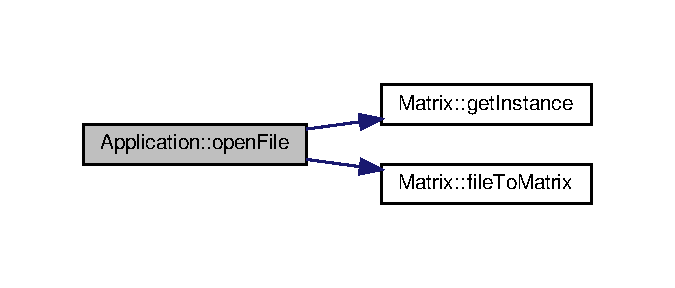
\includegraphics[width=324pt]{class_application_ab2f161414a4e2f16e28321c192051006_cgraph}
\end{center}
\end{figure}
\mbox{\Hypertarget{class_application_a533bb50380401b3a7bfaef31a9faf7f5}\label{class_application_a533bb50380401b3a7bfaef31a9faf7f5}} 
\index{Application@{Application}!save@{save}}
\index{save@{save}!Application@{Application}}
\subsubsection{\texorpdfstring{save()}{save()}}
{\footnotesize\ttfamily void Application\+::save (\begin{DoxyParamCaption}\item[{matrix}]{mat,  }\item[{string}]{filename }\end{DoxyParamCaption})}

Method accepting a matrix(probably an editted one) and is saving it to the same file. 
\begin{DoxyParams}{Parameters}
{\em mat} & \+: matrix \\
\hline
{\em filename} & \+: string \\
\hline
\end{DoxyParams}
\mbox{\Hypertarget{class_application_a26cc9a5dcdf0eebb9e89f6b3a8fa64dd}\label{class_application_a26cc9a5dcdf0eebb9e89f6b3a8fa64dd}} 
\index{Application@{Application}!save\+As@{save\+As}}
\index{save\+As@{save\+As}!Application@{Application}}
\subsubsection{\texorpdfstring{save\+As()}{saveAs()}}
{\footnotesize\ttfamily void Application\+::save\+As (\begin{DoxyParamCaption}\item[{matrix}]{mat }\end{DoxyParamCaption})}

Method accepting a matrix(probably and editted one) and is saving it to a new file. The user should enter the name of the new file. 
\begin{DoxyParams}{Parameters}
{\em mat} & \+: matrix \\
\hline
\end{DoxyParams}
\mbox{\Hypertarget{class_application_a76de879568ee39ac80484441716928d2}\label{class_application_a76de879568ee39ac80484441716928d2}} 
\index{Application@{Application}!set\+Filename@{set\+Filename}}
\index{set\+Filename@{set\+Filename}!Application@{Application}}
\subsubsection{\texorpdfstring{set\+Filename()}{setFilename()}}
{\footnotesize\ttfamily void Application\+::set\+Filename (\begin{DoxyParamCaption}\item[{const string \&}]{fname }\end{DoxyParamCaption})}

Methdd setting the filename. 
\begin{DoxyParams}{Parameters}
{\em fname} & \+: string \\
\hline
\end{DoxyParams}
\mbox{\Hypertarget{class_application_a56b4a55e9eabd40b7f0033ba39631ebe}\label{class_application_a56b4a55e9eabd40b7f0033ba39631ebe}} 
\index{Application@{Application}!set\+Matrix@{set\+Matrix}}
\index{set\+Matrix@{set\+Matrix}!Application@{Application}}
\subsubsection{\texorpdfstring{set\+Matrix()}{setMatrix()}}
{\footnotesize\ttfamily void Application\+::set\+Matrix (\begin{DoxyParamCaption}\item[{matrix}]{m }\end{DoxyParamCaption})}

Method setting the matrix. 
\begin{DoxyParams}{Parameters}
{\em m} & \+: matrix \\
\hline
\end{DoxyParams}


The documentation for this class was generated from the following files\+:\begin{DoxyCompactItemize}
\item 
application.\+h\item 
application.\+cpp\end{DoxyCompactItemize}

\hypertarget{class_formula}{}\section{Formula Class Reference}
\label{class_formula}\index{Formula@{Formula}}


The \hyperlink{class_formula}{Formula} class is used for editing a cell with a formula.  




{\ttfamily \#include $<$formula.\+h$>$}



Collaboration diagram for Formula\+:\nopagebreak
\begin{figure}[H]
\begin{center}
\leavevmode
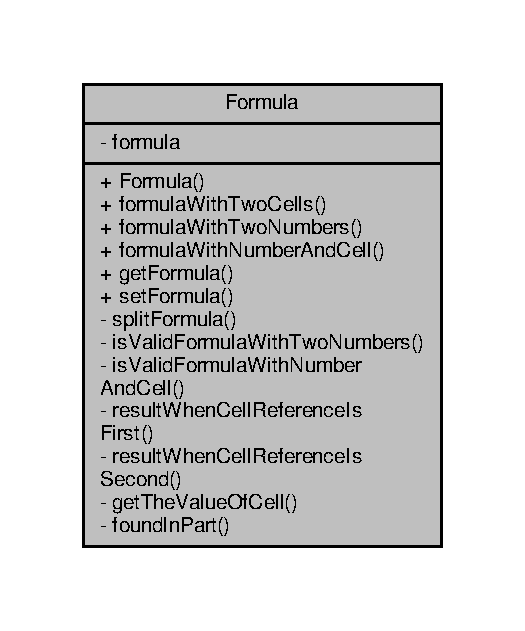
\includegraphics[width=252pt]{class_formula__coll__graph}
\end{center}
\end{figure}
\subsection*{Public Member Functions}
\begin{DoxyCompactItemize}
\item 
\hyperlink{class_formula_aed38ad076eb638148bcbe867d6acea60}{Formula} (string form)
\item 
double \hyperlink{class_formula_a518bc97bd50f1cc5573be7d3f8cb6253}{formula\+With\+Two\+Cells} (const matrix \&mat)
\item 
double \hyperlink{class_formula_a2159ffdb34d80f2bee422eee89fc871a}{formula\+With\+Two\+Numbers} ()
\item 
double \hyperlink{class_formula_a0f831b2ee98fbeb7df371f83ee7d374d}{formula\+With\+Number\+And\+Cell} (const matrix \&mat)
\item 
const string \& \hyperlink{class_formula_a1b9557287ed502f9523c5c7b1805bac1}{get\+Formula} () const
\item 
void \hyperlink{class_formula_aba7633655dad414ed0a1d92cdba38163}{set\+Formula} (const string \&formula)
\end{DoxyCompactItemize}
\subsection*{Private Member Functions}
\begin{DoxyCompactItemize}
\item 
void \hyperlink{class_formula_ae9390fbc99e5ade644589b144c73bfb7}{split\+Formula} (const string \&formula, string \&first\+Part, string \&second\+Part, int \&p)
\item 
bool \hyperlink{class_formula_a0a2b13b0f741ea650e1ae71269dde9a5}{is\+Valid\+Formula\+With\+Two\+Numbers} ()
\item 
bool \hyperlink{class_formula_a83eff8c83a0ea79b3dd21c2e86a546c8}{is\+Valid\+Formula\+With\+Number\+And\+Cell} ()
\item 
double \hyperlink{class_formula_a9a27ccdd3ee3143b1f6e541ec3c6a0ec}{result\+When\+Cell\+Reference\+Is\+First} (const matrix \&mat, string formula, const string \&first\+Part\+Of\+Formula, const string \&second\+Part\+Of\+Formula, int pos)
\item 
double \hyperlink{class_formula_ae0edae33b4af295bab04f1f1c06f406f}{result\+When\+Cell\+Reference\+Is\+Second} (const matrix \&mat, string formula, const string \&first\+Part\+Of\+Formula, const string \&second\+Part\+Of\+Formula, int pos)
\item 
double \hyperlink{class_formula_a8080ff3cf8fce2d9f1730e772ae21c71}{get\+The\+Value\+Of\+Cell} (const matrix \&mat, int row, int col)
\item 
bool \hyperlink{class_formula_a79079cea46f8320cd7a63f576251baac}{found\+In\+Part} (const string \&str)
\end{DoxyCompactItemize}
\subsection*{Private Attributes}
\begin{DoxyCompactItemize}
\item 
\mbox{\Hypertarget{class_formula_a2a3b5b998b48db1fadf57752e59ed4fb}\label{class_formula_a2a3b5b998b48db1fadf57752e59ed4fb}} 
string {\bfseries formula}
\end{DoxyCompactItemize}


\subsection{Detailed Description}
The \hyperlink{class_formula}{Formula} class is used for editing a cell with a formula. 

This class is used to initialize a formula and to read(decipher) it. There are three types of formulas\+: ~\newline

\begin{DoxyEnumerate}
\item number -\/ operator -\/ number ( = 10 $^\wedge$ 2 );
\item reference to a cell -\/ operator -\/ number ( = R1\+C1 / 5 );~\newline
 number -\/ operator -\/ reference to a cell ( = 5 $\ast$ R1\+C1 );
\item reference to a cell -\/ operator -\/ reference to a cell ( = R2\+C2 -\/ R3\+C4 );
\end{DoxyEnumerate}


\begin{DoxyParams}{Parameters}
{\em string} & fomrula \\
\hline
\end{DoxyParams}


\subsection{Constructor \& Destructor Documentation}
\mbox{\Hypertarget{class_formula_aed38ad076eb638148bcbe867d6acea60}\label{class_formula_aed38ad076eb638148bcbe867d6acea60}} 
\index{Formula@{Formula}!Formula@{Formula}}
\index{Formula@{Formula}!Formula@{Formula}}
\subsubsection{\texorpdfstring{Formula()}{Formula()}}
{\footnotesize\ttfamily Formula\+::\+Formula (\begin{DoxyParamCaption}\item[{string}]{form }\end{DoxyParamCaption})\hspace{0.3cm}{\ttfamily [inline]}}

A parametrized constructor. 
\begin{DoxyParams}{Parameters}
{\em form} & \\
\hline
\end{DoxyParams}


\subsection{Member Function Documentation}
\mbox{\Hypertarget{class_formula_a0f831b2ee98fbeb7df371f83ee7d374d}\label{class_formula_a0f831b2ee98fbeb7df371f83ee7d374d}} 
\index{Formula@{Formula}!formula\+With\+Number\+And\+Cell@{formula\+With\+Number\+And\+Cell}}
\index{formula\+With\+Number\+And\+Cell@{formula\+With\+Number\+And\+Cell}!Formula@{Formula}}
\subsubsection{\texorpdfstring{formula\+With\+Number\+And\+Cell()}{formulaWithNumberAndCell()}}
{\footnotesize\ttfamily double Formula\+::formula\+With\+Number\+And\+Cell (\begin{DoxyParamCaption}\item[{const matrix \&}]{mat }\end{DoxyParamCaption})}

Method calculating the value of formula with a number and a refenrence to a cell. 
\begin{DoxyParams}{Parameters}
{\em mat} & \\
\hline
\end{DoxyParams}
\begin{DoxyReturn}{Returns}

\end{DoxyReturn}
Here is the call graph for this function\+:\nopagebreak
\begin{figure}[H]
\begin{center}
\leavevmode
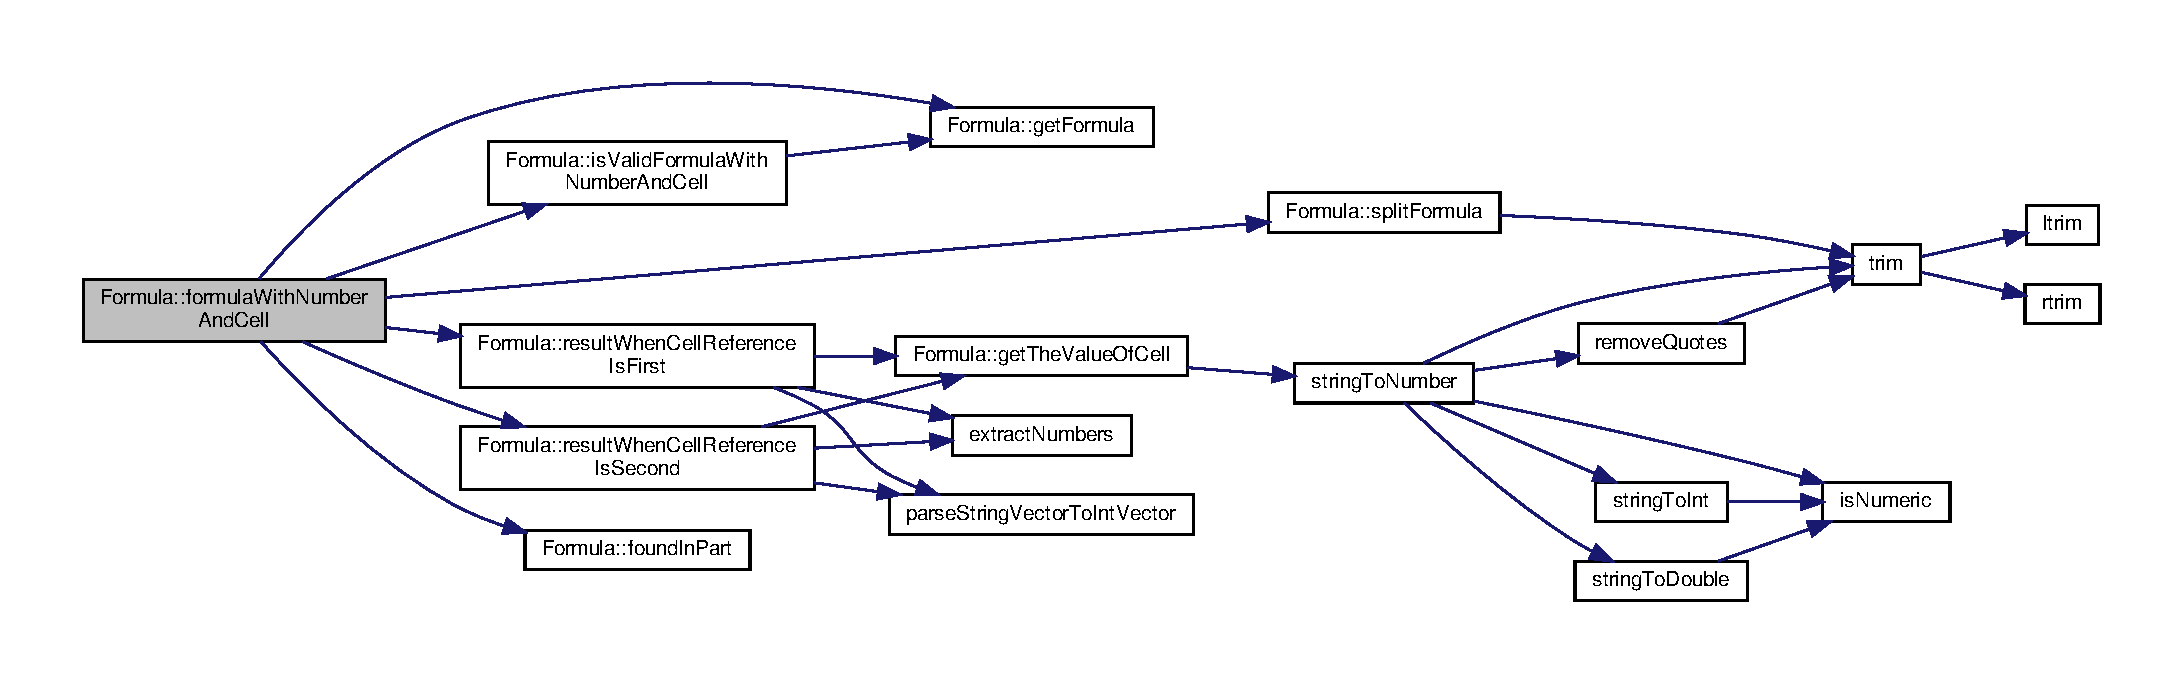
\includegraphics[width=350pt]{class_formula_a0f831b2ee98fbeb7df371f83ee7d374d_cgraph}
\end{center}
\end{figure}
Here is the caller graph for this function\+:\nopagebreak
\begin{figure}[H]
\begin{center}
\leavevmode
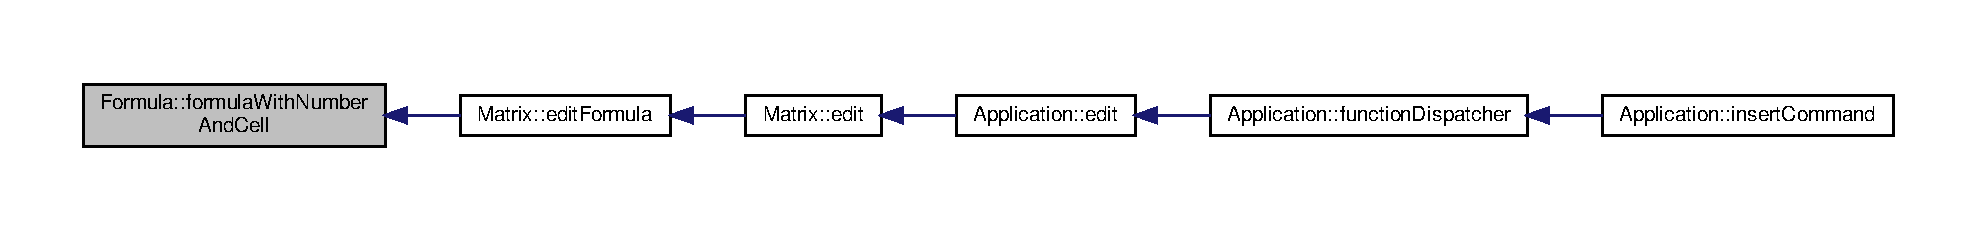
\includegraphics[width=350pt]{class_formula_a0f831b2ee98fbeb7df371f83ee7d374d_icgraph}
\end{center}
\end{figure}
\mbox{\Hypertarget{class_formula_a518bc97bd50f1cc5573be7d3f8cb6253}\label{class_formula_a518bc97bd50f1cc5573be7d3f8cb6253}} 
\index{Formula@{Formula}!formula\+With\+Two\+Cells@{formula\+With\+Two\+Cells}}
\index{formula\+With\+Two\+Cells@{formula\+With\+Two\+Cells}!Formula@{Formula}}
\subsubsection{\texorpdfstring{formula\+With\+Two\+Cells()}{formulaWithTwoCells()}}
{\footnotesize\ttfamily double Formula\+::formula\+With\+Two\+Cells (\begin{DoxyParamCaption}\item[{const matrix \&}]{mat }\end{DoxyParamCaption})}

Method calculating the value of formula with two references to a cell. 
\begin{DoxyParams}{Parameters}
{\em mat} & \\
\hline
\end{DoxyParams}
\begin{DoxyReturn}{Returns}
double 
\end{DoxyReturn}
Here is the call graph for this function\+:\nopagebreak
\begin{figure}[H]
\begin{center}
\leavevmode
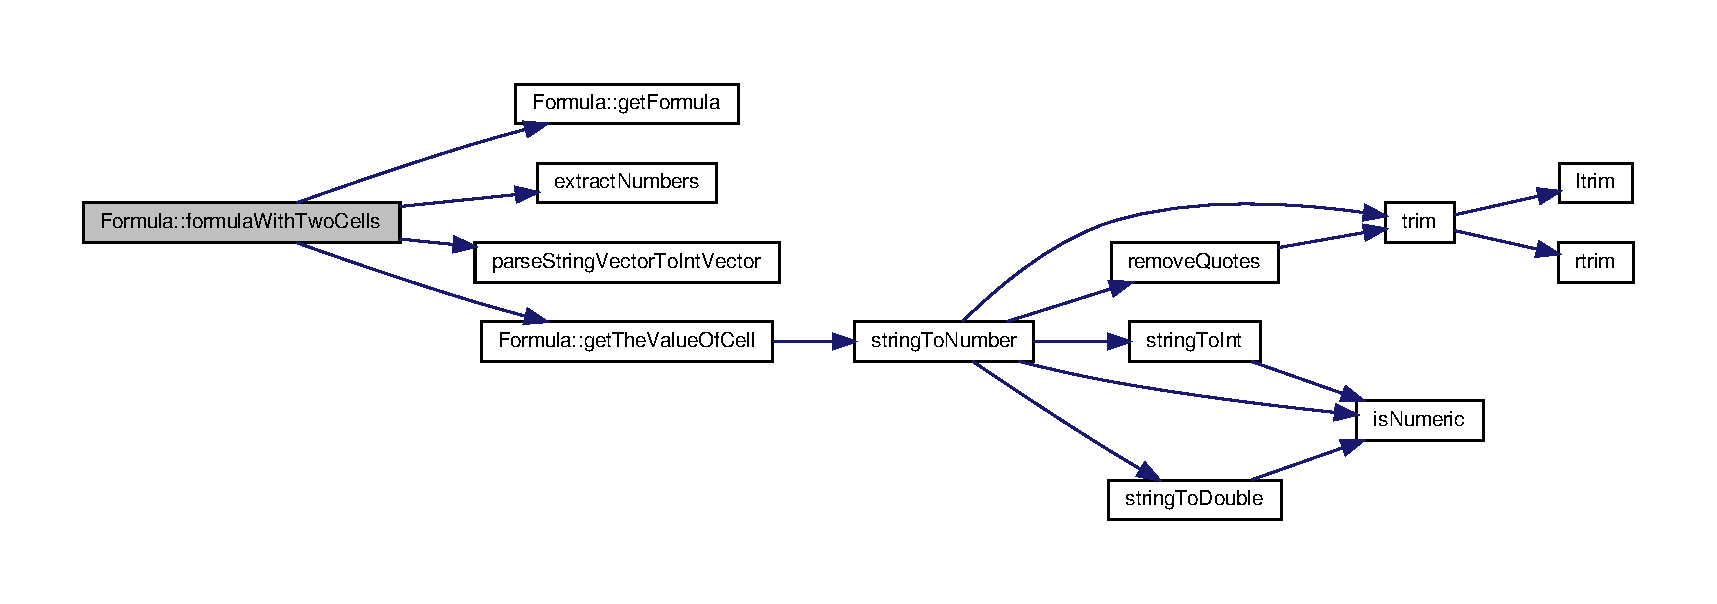
\includegraphics[width=350pt]{class_formula_a518bc97bd50f1cc5573be7d3f8cb6253_cgraph}
\end{center}
\end{figure}
Here is the caller graph for this function\+:\nopagebreak
\begin{figure}[H]
\begin{center}
\leavevmode
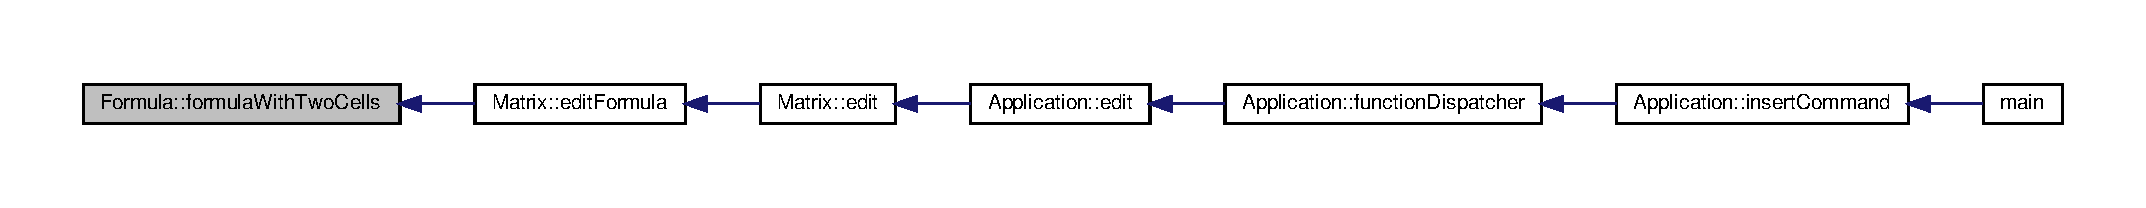
\includegraphics[width=350pt]{class_formula_a518bc97bd50f1cc5573be7d3f8cb6253_icgraph}
\end{center}
\end{figure}
\mbox{\Hypertarget{class_formula_a2159ffdb34d80f2bee422eee89fc871a}\label{class_formula_a2159ffdb34d80f2bee422eee89fc871a}} 
\index{Formula@{Formula}!formula\+With\+Two\+Numbers@{formula\+With\+Two\+Numbers}}
\index{formula\+With\+Two\+Numbers@{formula\+With\+Two\+Numbers}!Formula@{Formula}}
\subsubsection{\texorpdfstring{formula\+With\+Two\+Numbers()}{formulaWithTwoNumbers()}}
{\footnotesize\ttfamily double Formula\+::formula\+With\+Two\+Numbers (\begin{DoxyParamCaption}{ }\end{DoxyParamCaption})}

Method calculating the value of formula with two numbers. \begin{DoxyReturn}{Returns}
double 
\end{DoxyReturn}
Here is the call graph for this function\+:\nopagebreak
\begin{figure}[H]
\begin{center}
\leavevmode
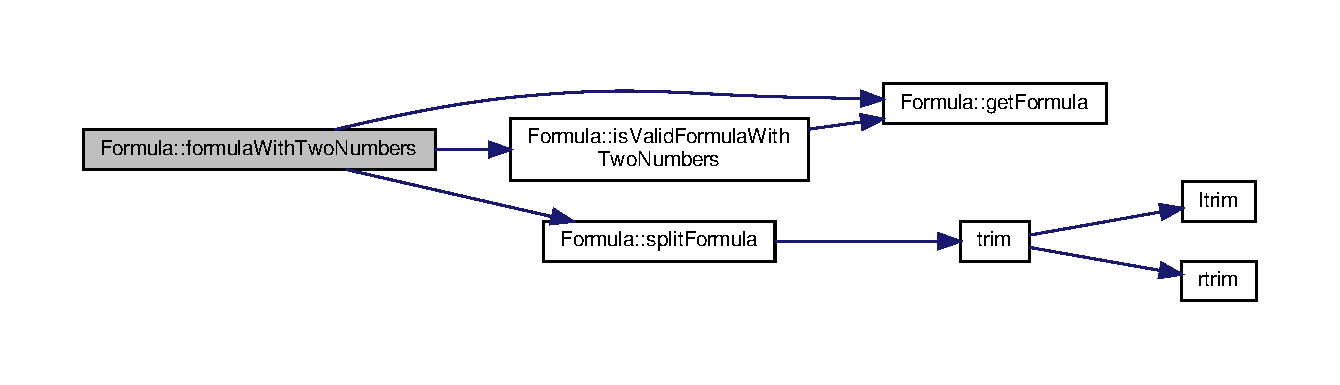
\includegraphics[width=350pt]{class_formula_a2159ffdb34d80f2bee422eee89fc871a_cgraph}
\end{center}
\end{figure}
Here is the caller graph for this function\+:\nopagebreak
\begin{figure}[H]
\begin{center}
\leavevmode
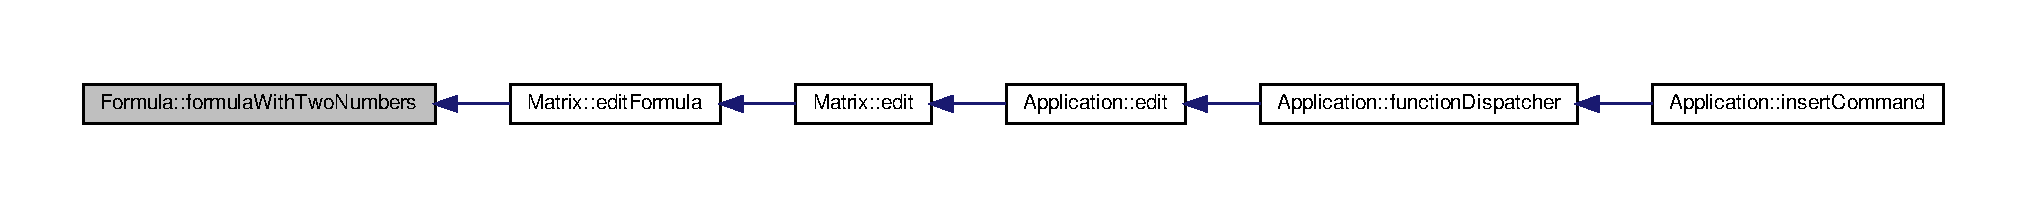
\includegraphics[width=350pt]{class_formula_a2159ffdb34d80f2bee422eee89fc871a_icgraph}
\end{center}
\end{figure}
\mbox{\Hypertarget{class_formula_a79079cea46f8320cd7a63f576251baac}\label{class_formula_a79079cea46f8320cd7a63f576251baac}} 
\index{Formula@{Formula}!found\+In\+Part@{found\+In\+Part}}
\index{found\+In\+Part@{found\+In\+Part}!Formula@{Formula}}
\subsubsection{\texorpdfstring{found\+In\+Part()}{foundInPart()}}
{\footnotesize\ttfamily bool Formula\+::found\+In\+Part (\begin{DoxyParamCaption}\item[{const string \&}]{str }\end{DoxyParamCaption})\hspace{0.3cm}{\ttfamily [private]}}

Used to determine in which part of the formula is the reference to a cell. 
\begin{DoxyParams}{Parameters}
{\em str} & \\
\hline
\end{DoxyParams}
\begin{DoxyReturn}{Returns}
true or false 
\end{DoxyReturn}
Here is the caller graph for this function\+:\nopagebreak
\begin{figure}[H]
\begin{center}
\leavevmode
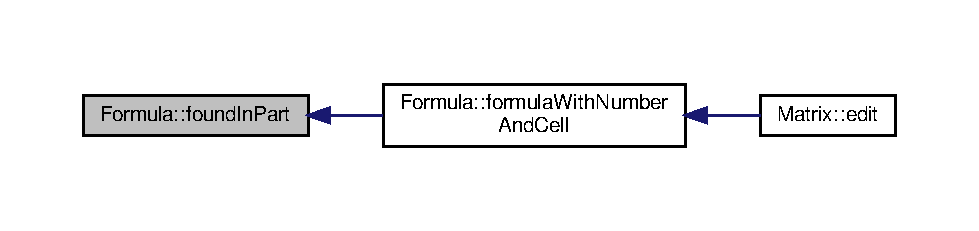
\includegraphics[width=350pt]{class_formula_a79079cea46f8320cd7a63f576251baac_icgraph}
\end{center}
\end{figure}
\mbox{\Hypertarget{class_formula_a1b9557287ed502f9523c5c7b1805bac1}\label{class_formula_a1b9557287ed502f9523c5c7b1805bac1}} 
\index{Formula@{Formula}!get\+Formula@{get\+Formula}}
\index{get\+Formula@{get\+Formula}!Formula@{Formula}}
\subsubsection{\texorpdfstring{get\+Formula()}{getFormula()}}
{\footnotesize\ttfamily const string \& Formula\+::get\+Formula (\begin{DoxyParamCaption}{ }\end{DoxyParamCaption}) const}

Getter for a formula. \begin{DoxyReturn}{Returns}
formula 
\end{DoxyReturn}
Here is the caller graph for this function\+:\nopagebreak
\begin{figure}[H]
\begin{center}
\leavevmode
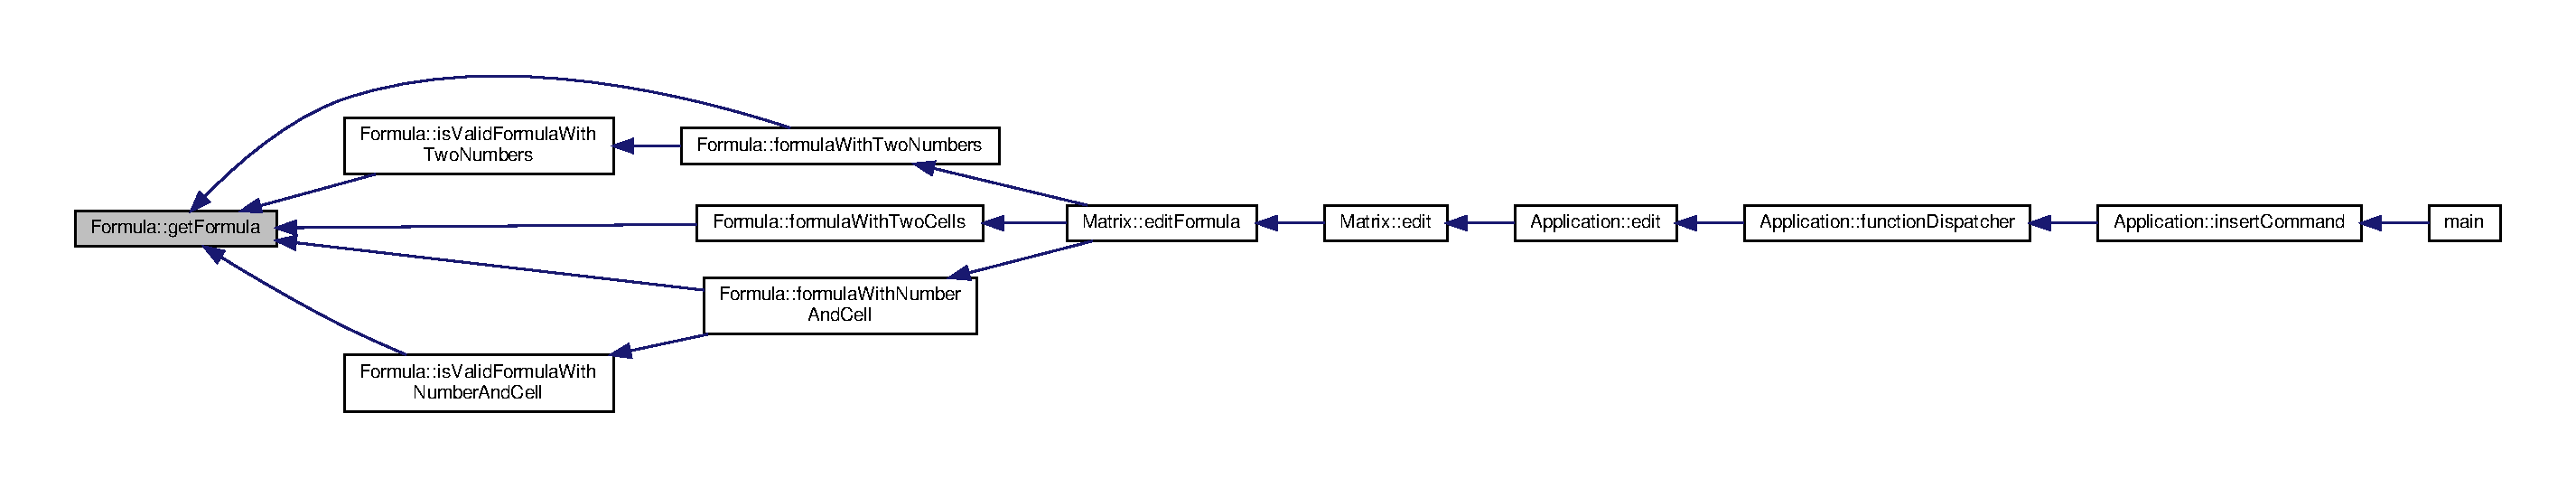
\includegraphics[width=350pt]{class_formula_a1b9557287ed502f9523c5c7b1805bac1_icgraph}
\end{center}
\end{figure}
\mbox{\Hypertarget{class_formula_a8080ff3cf8fce2d9f1730e772ae21c71}\label{class_formula_a8080ff3cf8fce2d9f1730e772ae21c71}} 
\index{Formula@{Formula}!get\+The\+Value\+Of\+Cell@{get\+The\+Value\+Of\+Cell}}
\index{get\+The\+Value\+Of\+Cell@{get\+The\+Value\+Of\+Cell}!Formula@{Formula}}
\subsubsection{\texorpdfstring{get\+The\+Value\+Of\+Cell()}{getTheValueOfCell()}}
{\footnotesize\ttfamily double Formula\+::get\+The\+Value\+Of\+Cell (\begin{DoxyParamCaption}\item[{const matrix \&}]{mat,  }\item[{int}]{row,  }\item[{int}]{col }\end{DoxyParamCaption})\hspace{0.3cm}{\ttfamily [private]}}

Accepts two integers(one for row and one for column) and extracts the value of the cell references with these numbers. 
\begin{DoxyParams}{Parameters}
{\em mat} & \\
\hline
{\em row} & \\
\hline
{\em col} & \\
\hline
\end{DoxyParams}
\begin{DoxyReturn}{Returns}

\end{DoxyReturn}
Here is the call graph for this function\+:\nopagebreak
\begin{figure}[H]
\begin{center}
\leavevmode
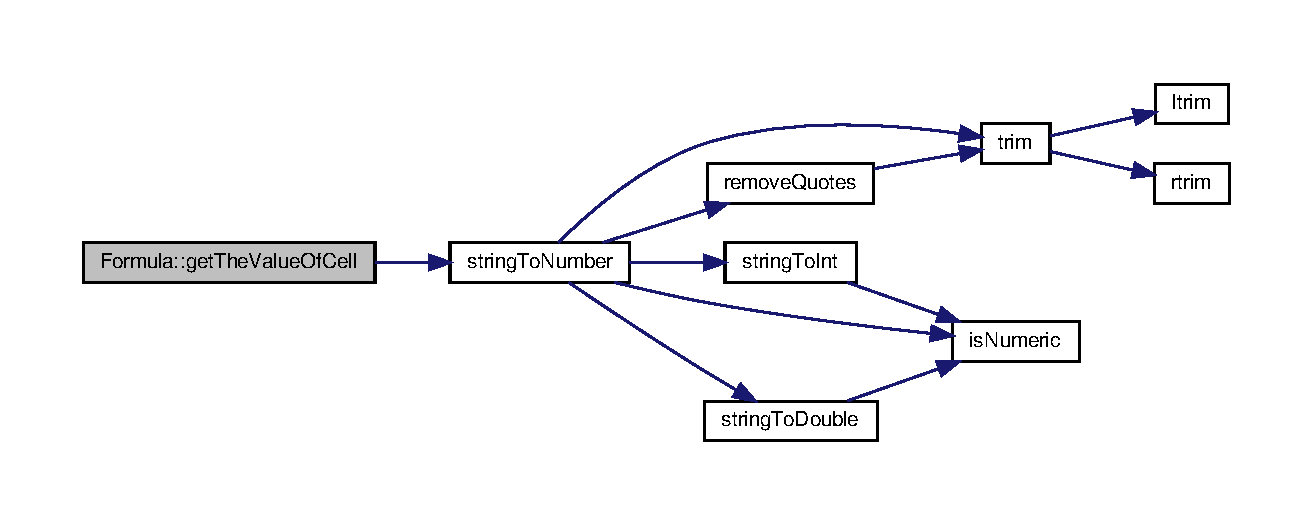
\includegraphics[width=350pt]{class_formula_a8080ff3cf8fce2d9f1730e772ae21c71_cgraph}
\end{center}
\end{figure}
Here is the caller graph for this function\+:\nopagebreak
\begin{figure}[H]
\begin{center}
\leavevmode
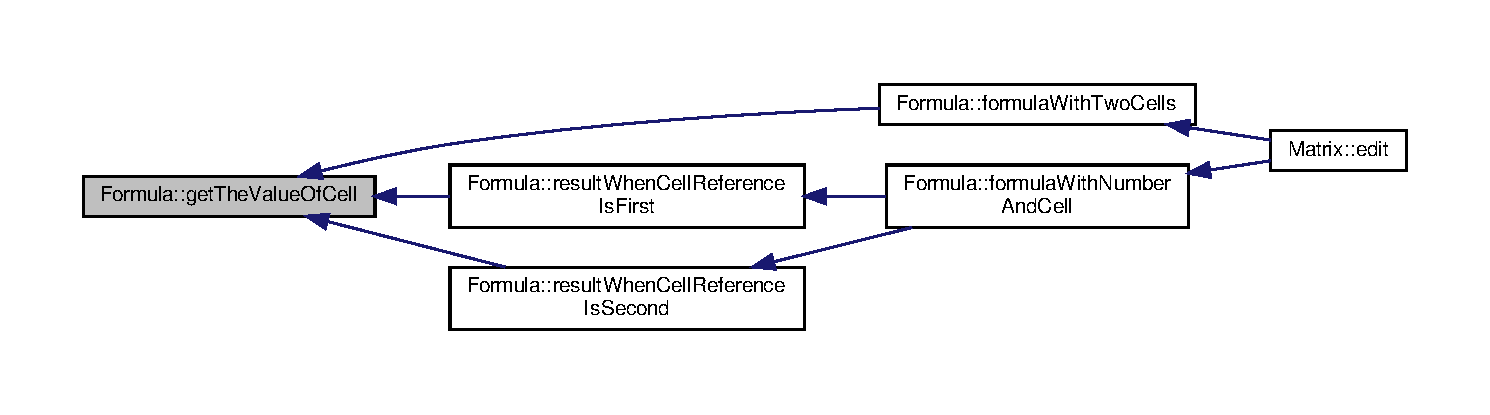
\includegraphics[width=350pt]{class_formula_a8080ff3cf8fce2d9f1730e772ae21c71_icgraph}
\end{center}
\end{figure}
\mbox{\Hypertarget{class_formula_a83eff8c83a0ea79b3dd21c2e86a546c8}\label{class_formula_a83eff8c83a0ea79b3dd21c2e86a546c8}} 
\index{Formula@{Formula}!is\+Valid\+Formula\+With\+Number\+And\+Cell@{is\+Valid\+Formula\+With\+Number\+And\+Cell}}
\index{is\+Valid\+Formula\+With\+Number\+And\+Cell@{is\+Valid\+Formula\+With\+Number\+And\+Cell}!Formula@{Formula}}
\subsubsection{\texorpdfstring{is\+Valid\+Formula\+With\+Number\+And\+Cell()}{isValidFormulaWithNumberAndCell()}}
{\footnotesize\ttfamily bool Formula\+::is\+Valid\+Formula\+With\+Number\+And\+Cell (\begin{DoxyParamCaption}{ }\end{DoxyParamCaption})\hspace{0.3cm}{\ttfamily [private]}}

Checks whether the formula with a number and a reference to a cell is valid. \begin{DoxyReturn}{Returns}
true or false 
\end{DoxyReturn}
Here is the call graph for this function\+:\nopagebreak
\begin{figure}[H]
\begin{center}
\leavevmode
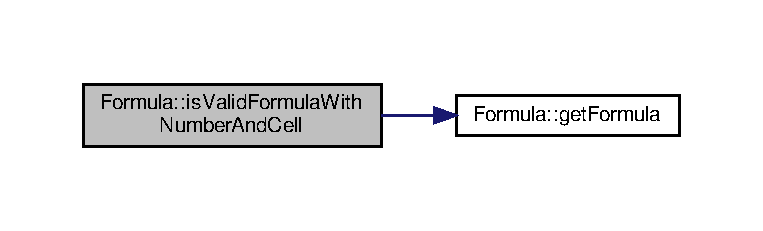
\includegraphics[width=350pt]{class_formula_a83eff8c83a0ea79b3dd21c2e86a546c8_cgraph}
\end{center}
\end{figure}
Here is the caller graph for this function\+:\nopagebreak
\begin{figure}[H]
\begin{center}
\leavevmode
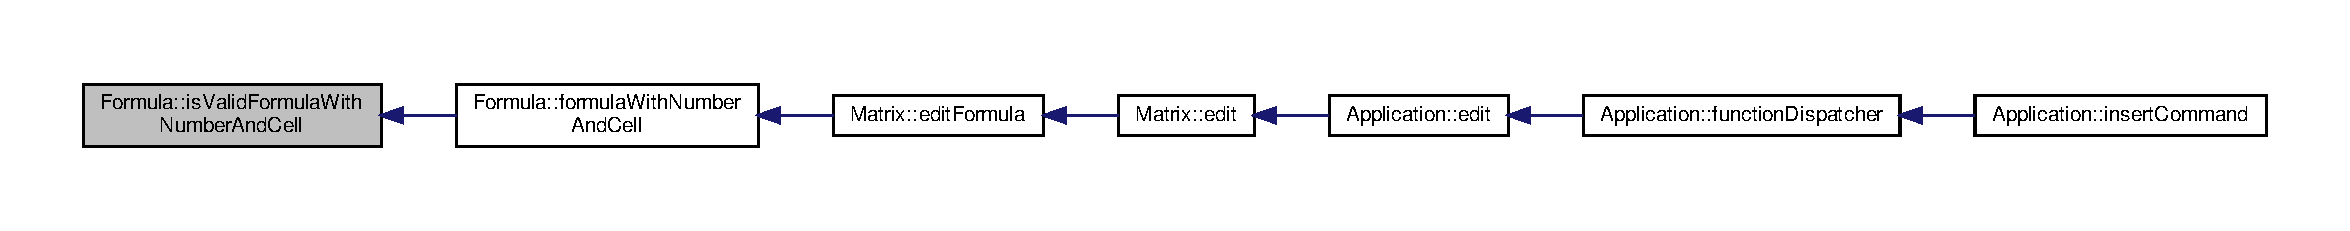
\includegraphics[width=350pt]{class_formula_a83eff8c83a0ea79b3dd21c2e86a546c8_icgraph}
\end{center}
\end{figure}
\mbox{\Hypertarget{class_formula_a0a2b13b0f741ea650e1ae71269dde9a5}\label{class_formula_a0a2b13b0f741ea650e1ae71269dde9a5}} 
\index{Formula@{Formula}!is\+Valid\+Formula\+With\+Two\+Numbers@{is\+Valid\+Formula\+With\+Two\+Numbers}}
\index{is\+Valid\+Formula\+With\+Two\+Numbers@{is\+Valid\+Formula\+With\+Two\+Numbers}!Formula@{Formula}}
\subsubsection{\texorpdfstring{is\+Valid\+Formula\+With\+Two\+Numbers()}{isValidFormulaWithTwoNumbers()}}
{\footnotesize\ttfamily bool Formula\+::is\+Valid\+Formula\+With\+Two\+Numbers (\begin{DoxyParamCaption}{ }\end{DoxyParamCaption})\hspace{0.3cm}{\ttfamily [private]}}

Checks whether the formula with two numbers is valid. \begin{DoxyReturn}{Returns}
true or false 
\end{DoxyReturn}
Here is the call graph for this function\+:\nopagebreak
\begin{figure}[H]
\begin{center}
\leavevmode
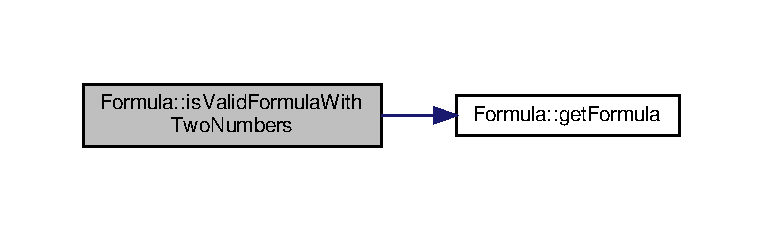
\includegraphics[width=350pt]{class_formula_a0a2b13b0f741ea650e1ae71269dde9a5_cgraph}
\end{center}
\end{figure}
Here is the caller graph for this function\+:\nopagebreak
\begin{figure}[H]
\begin{center}
\leavevmode
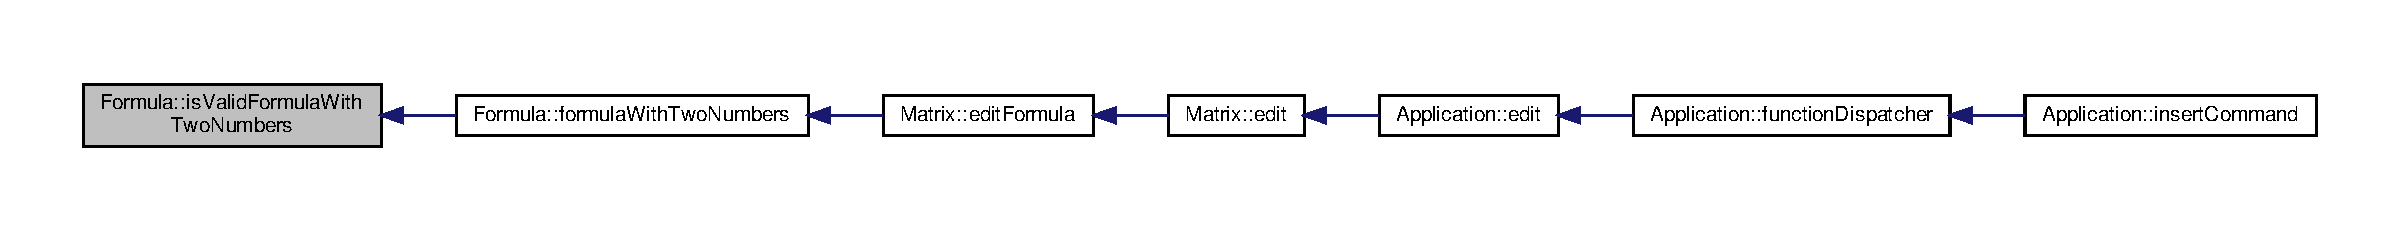
\includegraphics[width=350pt]{class_formula_a0a2b13b0f741ea650e1ae71269dde9a5_icgraph}
\end{center}
\end{figure}
\mbox{\Hypertarget{class_formula_a9a27ccdd3ee3143b1f6e541ec3c6a0ec}\label{class_formula_a9a27ccdd3ee3143b1f6e541ec3c6a0ec}} 
\index{Formula@{Formula}!result\+When\+Cell\+Reference\+Is\+First@{result\+When\+Cell\+Reference\+Is\+First}}
\index{result\+When\+Cell\+Reference\+Is\+First@{result\+When\+Cell\+Reference\+Is\+First}!Formula@{Formula}}
\subsubsection{\texorpdfstring{result\+When\+Cell\+Reference\+Is\+First()}{resultWhenCellReferenceIsFirst()}}
{\footnotesize\ttfamily double Formula\+::result\+When\+Cell\+Reference\+Is\+First (\begin{DoxyParamCaption}\item[{const matrix \&}]{mat,  }\item[{string}]{formula,  }\item[{const string \&}]{first\+Part\+Of\+Formula,  }\item[{const string \&}]{second\+Part\+Of\+Formula,  }\item[{int}]{pos }\end{DoxyParamCaption})\hspace{0.3cm}{\ttfamily [private]}}

Returning the result from the formula when the reference is first in the formula. 
\begin{DoxyParams}{Parameters}
{\em mat} & \\
\hline
{\em formula} & \\
\hline
{\em first\+Part\+Of\+Formula} & \\
\hline
{\em second\+Part\+Of\+Formula} & \\
\hline
{\em pos} & \\
\hline
\end{DoxyParams}
\begin{DoxyReturn}{Returns}
double 
\end{DoxyReturn}
Here is the call graph for this function\+:\nopagebreak
\begin{figure}[H]
\begin{center}
\leavevmode
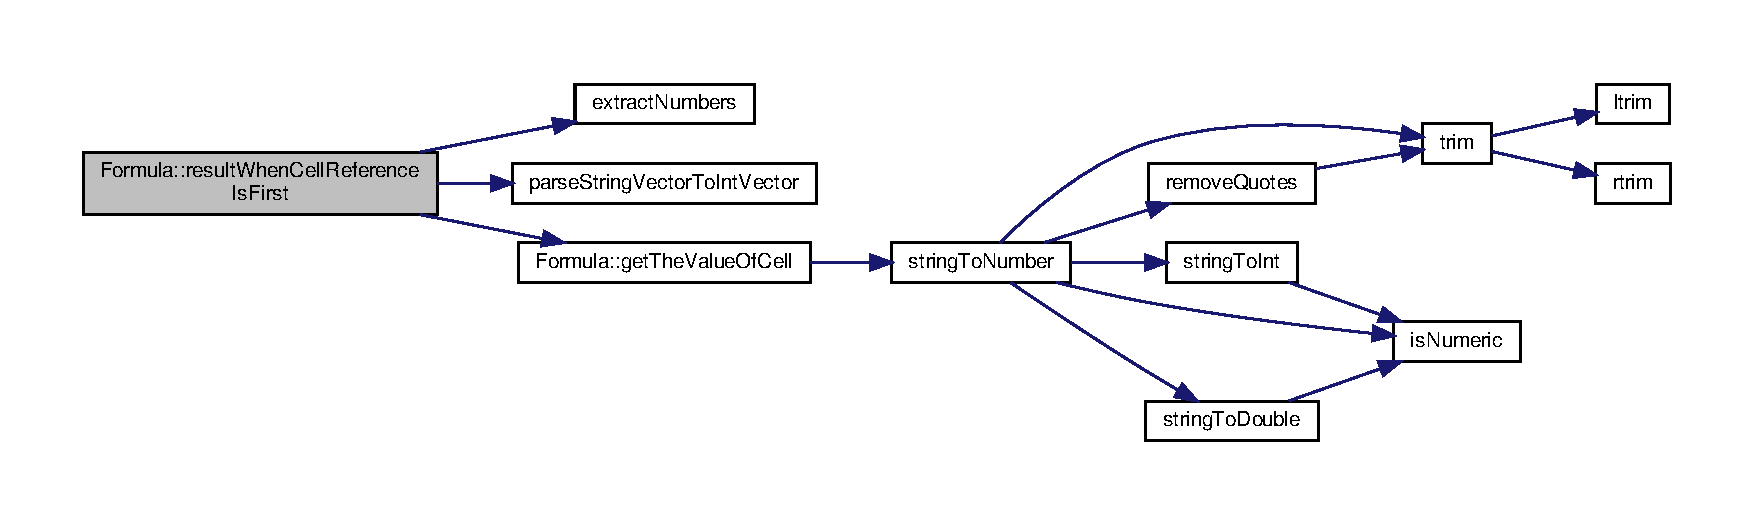
\includegraphics[width=350pt]{class_formula_a9a27ccdd3ee3143b1f6e541ec3c6a0ec_cgraph}
\end{center}
\end{figure}
Here is the caller graph for this function\+:\nopagebreak
\begin{figure}[H]
\begin{center}
\leavevmode
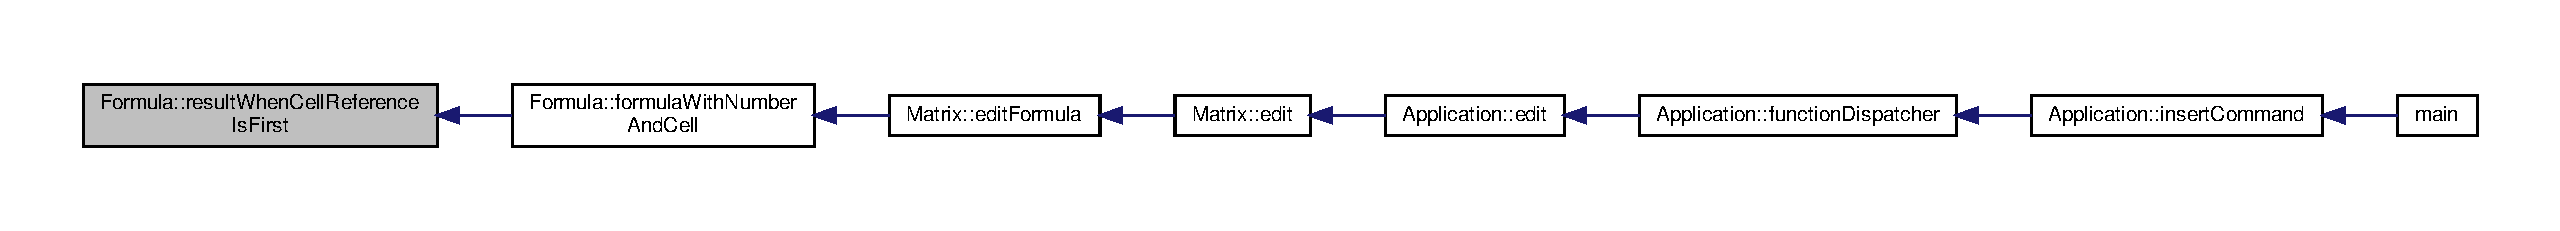
\includegraphics[width=350pt]{class_formula_a9a27ccdd3ee3143b1f6e541ec3c6a0ec_icgraph}
\end{center}
\end{figure}
\mbox{\Hypertarget{class_formula_ae0edae33b4af295bab04f1f1c06f406f}\label{class_formula_ae0edae33b4af295bab04f1f1c06f406f}} 
\index{Formula@{Formula}!result\+When\+Cell\+Reference\+Is\+Second@{result\+When\+Cell\+Reference\+Is\+Second}}
\index{result\+When\+Cell\+Reference\+Is\+Second@{result\+When\+Cell\+Reference\+Is\+Second}!Formula@{Formula}}
\subsubsection{\texorpdfstring{result\+When\+Cell\+Reference\+Is\+Second()}{resultWhenCellReferenceIsSecond()}}
{\footnotesize\ttfamily double Formula\+::result\+When\+Cell\+Reference\+Is\+Second (\begin{DoxyParamCaption}\item[{const matrix \&}]{mat,  }\item[{string}]{formula,  }\item[{const string \&}]{first\+Part\+Of\+Formula,  }\item[{const string \&}]{second\+Part\+Of\+Formula,  }\item[{int}]{pos }\end{DoxyParamCaption})\hspace{0.3cm}{\ttfamily [private]}}

Returning the result from the formula when the reference is second in the formula. 
\begin{DoxyParams}{Parameters}
{\em mat} & \\
\hline
{\em formula} & \\
\hline
{\em first\+Part\+Of\+Formula} & \\
\hline
{\em second\+Part\+Of\+Formula} & \\
\hline
{\em pos} & \\
\hline
\end{DoxyParams}
\begin{DoxyReturn}{Returns}
double 
\end{DoxyReturn}
Here is the call graph for this function\+:\nopagebreak
\begin{figure}[H]
\begin{center}
\leavevmode
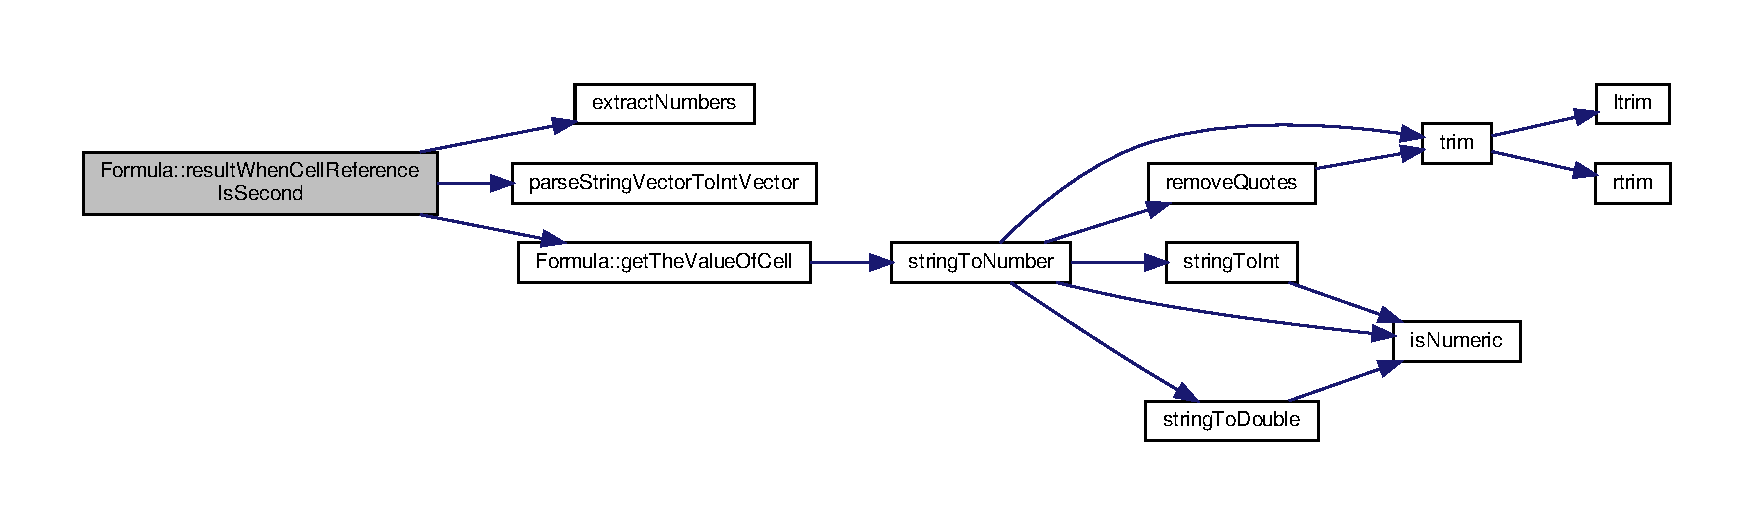
\includegraphics[width=350pt]{class_formula_ae0edae33b4af295bab04f1f1c06f406f_cgraph}
\end{center}
\end{figure}
Here is the caller graph for this function\+:\nopagebreak
\begin{figure}[H]
\begin{center}
\leavevmode
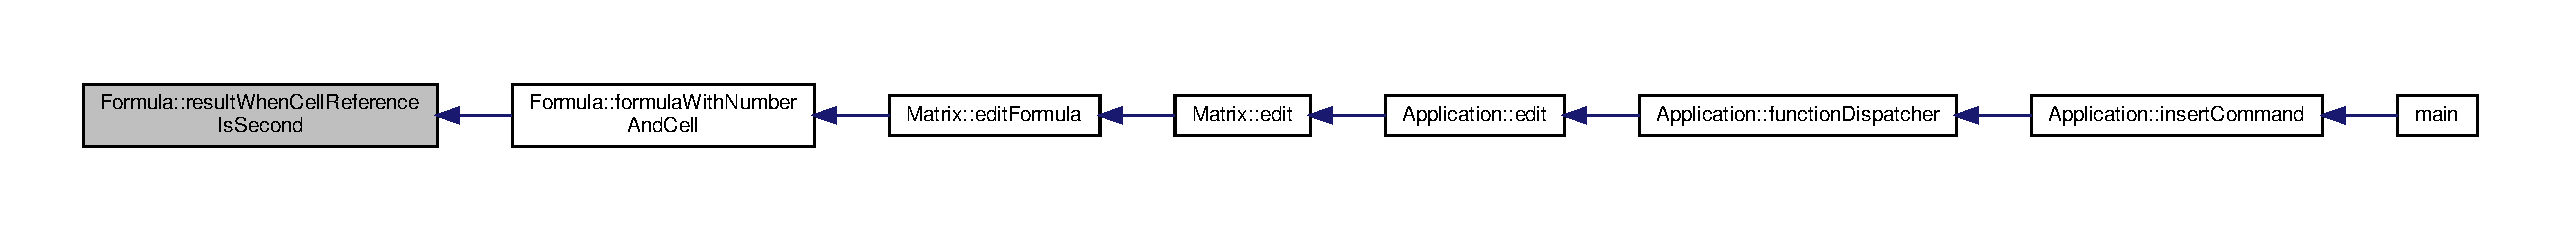
\includegraphics[width=350pt]{class_formula_ae0edae33b4af295bab04f1f1c06f406f_icgraph}
\end{center}
\end{figure}
\mbox{\Hypertarget{class_formula_aba7633655dad414ed0a1d92cdba38163}\label{class_formula_aba7633655dad414ed0a1d92cdba38163}} 
\index{Formula@{Formula}!set\+Formula@{set\+Formula}}
\index{set\+Formula@{set\+Formula}!Formula@{Formula}}
\subsubsection{\texorpdfstring{set\+Formula()}{setFormula()}}
{\footnotesize\ttfamily void Formula\+::set\+Formula (\begin{DoxyParamCaption}\item[{const string \&}]{formula }\end{DoxyParamCaption})}

Setter for a formula. 
\begin{DoxyParams}{Parameters}
{\em formula} & \\
\hline
\end{DoxyParams}
\mbox{\Hypertarget{class_formula_ae9390fbc99e5ade644589b144c73bfb7}\label{class_formula_ae9390fbc99e5ade644589b144c73bfb7}} 
\index{Formula@{Formula}!split\+Formula@{split\+Formula}}
\index{split\+Formula@{split\+Formula}!Formula@{Formula}}
\subsubsection{\texorpdfstring{split\+Formula()}{splitFormula()}}
{\footnotesize\ttfamily void Formula\+::split\+Formula (\begin{DoxyParamCaption}\item[{const string \&}]{formula,  }\item[{string \&}]{first\+Part,  }\item[{string \&}]{second\+Part,  }\item[{int \&}]{p }\end{DoxyParamCaption})\hspace{0.3cm}{\ttfamily [private]}}

This function is splitting the formula into two parts and the delimeter is the operator. 
\begin{DoxyParams}{Parameters}
{\em formula} & \\
\hline
{\em first\+Part} & \\
\hline
{\em second\+Part} & \\
\hline
{\em two} & strings \\
\hline
\end{DoxyParams}
Here is the call graph for this function\+:\nopagebreak
\begin{figure}[H]
\begin{center}
\leavevmode
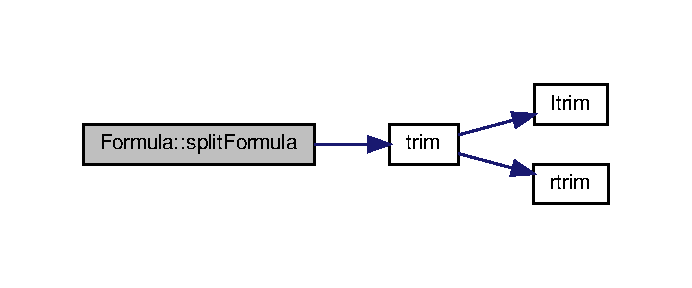
\includegraphics[width=332pt]{class_formula_ae9390fbc99e5ade644589b144c73bfb7_cgraph}
\end{center}
\end{figure}
Here is the caller graph for this function\+:\nopagebreak
\begin{figure}[H]
\begin{center}
\leavevmode
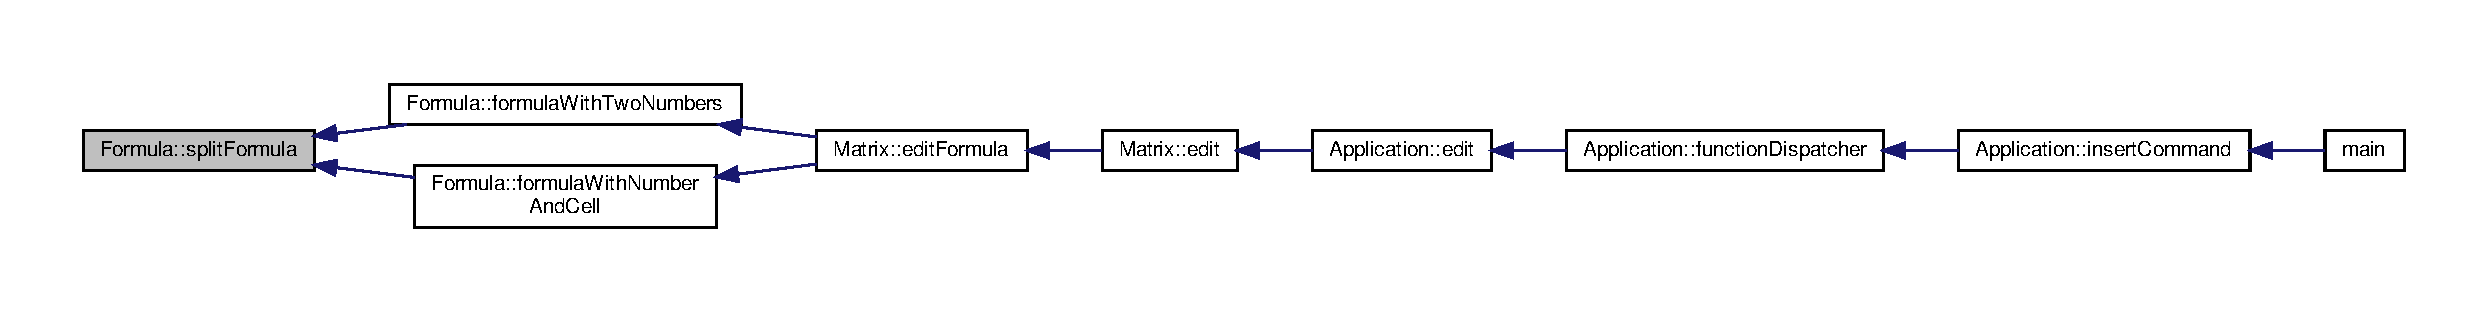
\includegraphics[width=350pt]{class_formula_ae9390fbc99e5ade644589b144c73bfb7_icgraph}
\end{center}
\end{figure}


The documentation for this class was generated from the following files\+:\begin{DoxyCompactItemize}
\item 
formula.\+h\item 
formula.\+cpp\end{DoxyCompactItemize}

\hypertarget{class_matrix}{}\section{Matrix Class Reference}
\label{class_matrix}\index{Matrix@{Matrix}}


A \hyperlink{class_matrix}{Matrix} class using a singleton design pattern.  




{\ttfamily \#include $<$matrix.\+h$>$}



Collaboration diagram for Matrix\+:
\nopagebreak
\begin{figure}[H]
\begin{center}
\leavevmode
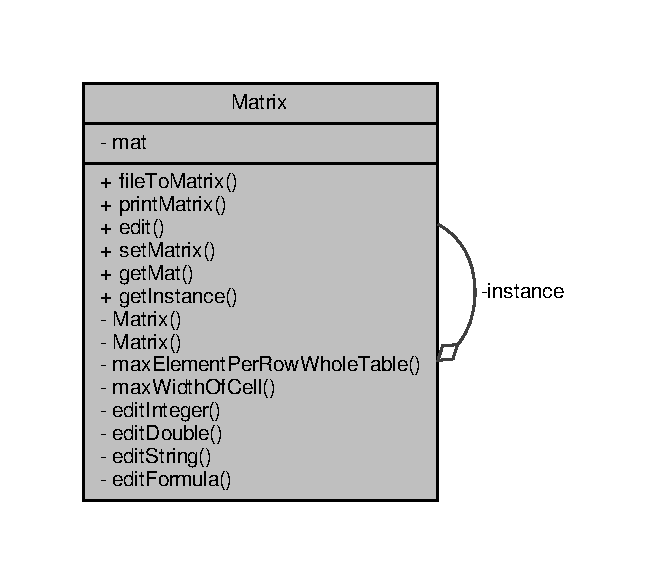
\includegraphics[width=311pt]{class_matrix__coll__graph}
\end{center}
\end{figure}
\subsection*{Public Member Functions}
\begin{DoxyCompactItemize}
\item 
\hyperlink{formula_8h_a869e2a5deeb3daa4c82d6bc91cf20d92}{matrix} \hyperlink{class_matrix_a35eb9dcb01c552fea1f5926db35339ef}{file\+To\+Matrix} (const string \&filename)
\item 
void \hyperlink{class_matrix_aa1967ad240a5ffaf492800044b7275d9}{print\+Matrix} ()
\item 
\hyperlink{formula_8h_a869e2a5deeb3daa4c82d6bc91cf20d92}{matrix} \hyperlink{class_matrix_a34b2269a2b6d06c202439de2e64009ba}{edit} (int row, int col)
\item 
void \hyperlink{class_matrix_a8c45dd1354fa25e14065cab23f3074c0}{set\+Matrix} (const \hyperlink{formula_8h_a869e2a5deeb3daa4c82d6bc91cf20d92}{matrix} \&\hyperlink{class_matrix_a1b0c75c45092426431308172aab92c66}{mat})
\item 
const \hyperlink{formula_8h_a869e2a5deeb3daa4c82d6bc91cf20d92}{matrix} \& \hyperlink{class_matrix_a52d82641f52304c9b6525747cd7f960c}{get\+Mat} () const
\end{DoxyCompactItemize}
\subsection*{Static Public Member Functions}
\begin{DoxyCompactItemize}
\item 
static \hyperlink{class_matrix}{Matrix} $\ast$ \hyperlink{class_matrix_a0c8e09a50ddb4d068d39456ea130abcc}{get\+Instance} ()
\end{DoxyCompactItemize}
\subsection*{Private Member Functions}
\begin{DoxyCompactItemize}
\item 
\hyperlink{class_matrix_a2dba13c45127354c9f75ef576f49269b}{Matrix} ()
\item 
\hyperlink{class_matrix_abc64f3d5a4f22323a24be2bfabf377cb}{Matrix} (\hyperlink{formula_8h_a869e2a5deeb3daa4c82d6bc91cf20d92}{matrix} m)
\item 
int \hyperlink{class_matrix_a8620c5426a31cf8fe0072df32bb3f65d}{max\+Element\+Per\+Row\+Whole\+Table} ()
\item 
int \hyperlink{class_matrix_a60dac9b70e73a12d2adb32d6be9ff65d}{max\+Width\+Of\+Cell} ()
\item 
\hyperlink{formula_8h_a869e2a5deeb3daa4c82d6bc91cf20d92}{matrix} \hyperlink{class_matrix_a91c66e2961a16adf56b8d58b916d2d46}{edit\+Integer} (int rol, int col)
\item 
\hyperlink{formula_8h_a869e2a5deeb3daa4c82d6bc91cf20d92}{matrix} \hyperlink{class_matrix_a147d3813e96ef757fb0d5ff65e5f97ef}{edit\+Double} (int rol, int col)
\item 
\hyperlink{formula_8h_a869e2a5deeb3daa4c82d6bc91cf20d92}{matrix} \hyperlink{class_matrix_a7029d8a3cd3c691b46adfd777abc880c}{edit\+String} (int rol, int col)
\item 
\hyperlink{formula_8h_a869e2a5deeb3daa4c82d6bc91cf20d92}{matrix} \hyperlink{class_matrix_af3d26e46fcec1a98380b1af04f008f22}{edit\+Formula} (int row, int col)
\end{DoxyCompactItemize}
\subsection*{Private Attributes}
\begin{DoxyCompactItemize}
\item 
\hyperlink{formula_8h_a869e2a5deeb3daa4c82d6bc91cf20d92}{matrix} \hyperlink{class_matrix_a1b0c75c45092426431308172aab92c66}{mat}
\end{DoxyCompactItemize}
\subsection*{Static Private Attributes}
\begin{DoxyCompactItemize}
\item 
static \hyperlink{class_matrix}{Matrix} $\ast$ \hyperlink{class_matrix_adbe13eefa6a6ea2f02f45da26400f22e}{instance} = 0
\end{DoxyCompactItemize}


\subsection{Detailed Description}
A \hyperlink{class_matrix}{Matrix} class using a singleton design pattern. 


\begin{DoxyParams}{Parameters}
{\em matrix} & mat \\
\hline
{\em static} & Matrix$\ast$ instance\\
\hline
\end{DoxyParams}
This class is used to initialize a matrix when opening a file. It uses a singleton pattern becasue after initializing a matrix the program is performing operations only on that particular matrix. That\textquotesingle{}s why we need just one instance of class \hyperlink{class_matrix}{Matrix}. 

\subsection{Constructor \& Destructor Documentation}
\mbox{\Hypertarget{class_matrix_a2dba13c45127354c9f75ef576f49269b}\label{class_matrix_a2dba13c45127354c9f75ef576f49269b}} 
\index{Matrix@{Matrix}!Matrix@{Matrix}}
\index{Matrix@{Matrix}!Matrix@{Matrix}}
\subsubsection{\texorpdfstring{Matrix()}{Matrix()}\hspace{0.1cm}{\footnotesize\ttfamily [1/2]}}
{\footnotesize\ttfamily Matrix\+::\+Matrix (\begin{DoxyParamCaption}{ }\end{DoxyParamCaption})\hspace{0.3cm}{\ttfamily [inline]}, {\ttfamily [private]}}

A default constructor. It is in the private section because the class uses singleton design pattern. \mbox{\Hypertarget{class_matrix_abc64f3d5a4f22323a24be2bfabf377cb}\label{class_matrix_abc64f3d5a4f22323a24be2bfabf377cb}} 
\index{Matrix@{Matrix}!Matrix@{Matrix}}
\index{Matrix@{Matrix}!Matrix@{Matrix}}
\subsubsection{\texorpdfstring{Matrix()}{Matrix()}\hspace{0.1cm}{\footnotesize\ttfamily [2/2]}}
{\footnotesize\ttfamily Matrix\+::\+Matrix (\begin{DoxyParamCaption}\item[{\hyperlink{formula_8h_a869e2a5deeb3daa4c82d6bc91cf20d92}{matrix}}]{m }\end{DoxyParamCaption})\hspace{0.3cm}{\ttfamily [inline]}, {\ttfamily [private]}}

A parametrized constructor. It is in the private section because the class uses singleton design pattern. 

\subsection{Member Function Documentation}
\mbox{\Hypertarget{class_matrix_a34b2269a2b6d06c202439de2e64009ba}\label{class_matrix_a34b2269a2b6d06c202439de2e64009ba}} 
\index{Matrix@{Matrix}!edit@{edit}}
\index{edit@{edit}!Matrix@{Matrix}}
\subsubsection{\texorpdfstring{edit()}{edit()}}
{\footnotesize\ttfamily \hyperlink{formula_8h_a869e2a5deeb3daa4c82d6bc91cf20d92}{matrix} Matrix\+::edit (\begin{DoxyParamCaption}\item[{int}]{row,  }\item[{int}]{col }\end{DoxyParamCaption})}

Method that is used to edit a cell in the matrix. It is accepting two integers(one for row and one for column). The user is asked to enter the desired data type for the cell that is going to be edited. He can choose from\+: integer, double, string or formula(= reference(to cell)/number -\/ operator -\/ reference(to cell)/number). 
\begin{DoxyParams}{Parameters}
{\em row} & \\
\hline
{\em col} & \\
\hline
\end{DoxyParams}
\begin{DoxyReturn}{Returns}
editted matrix 
\end{DoxyReturn}
Here is the call graph for this function\+:
\nopagebreak
\begin{figure}[H]
\begin{center}
\leavevmode
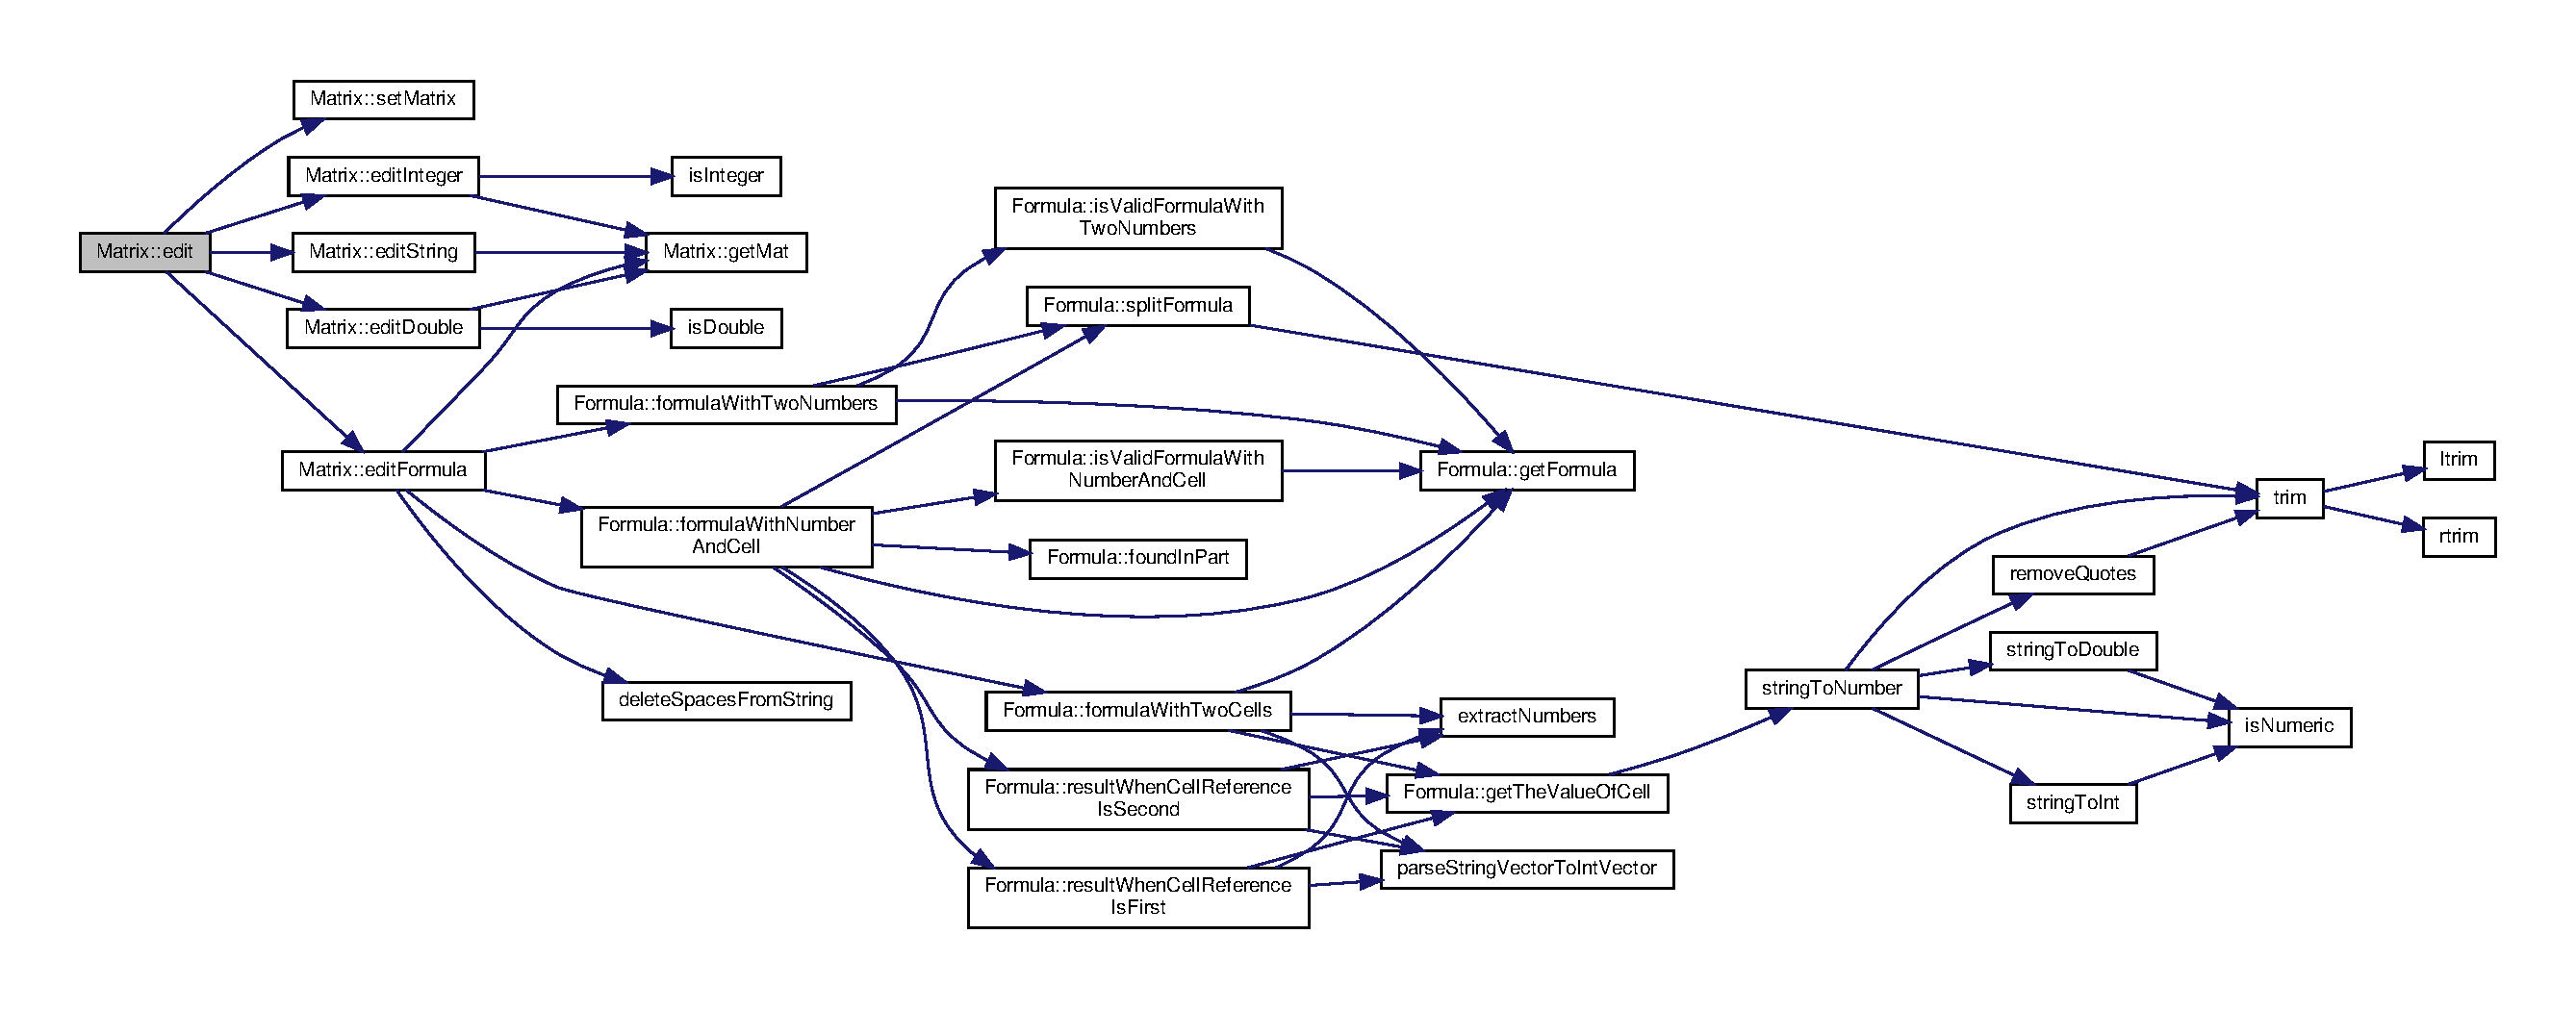
\includegraphics[width=350pt]{class_matrix_a34b2269a2b6d06c202439de2e64009ba_cgraph}
\end{center}
\end{figure}
Here is the caller graph for this function\+:
\nopagebreak
\begin{figure}[H]
\begin{center}
\leavevmode
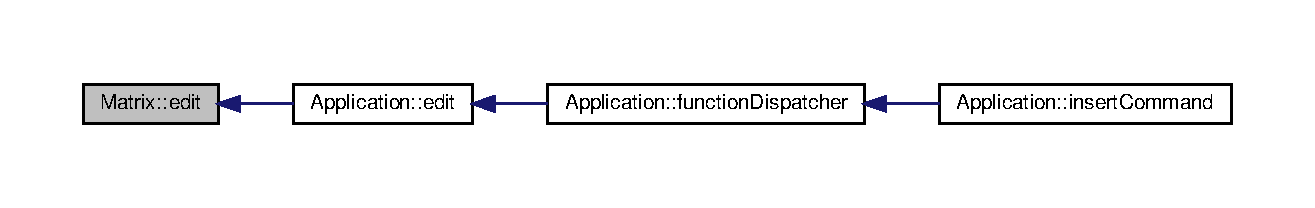
\includegraphics[width=350pt]{class_matrix_a34b2269a2b6d06c202439de2e64009ba_icgraph}
\end{center}
\end{figure}
\mbox{\Hypertarget{class_matrix_a147d3813e96ef757fb0d5ff65e5f97ef}\label{class_matrix_a147d3813e96ef757fb0d5ff65e5f97ef}} 
\index{Matrix@{Matrix}!edit\+Double@{edit\+Double}}
\index{edit\+Double@{edit\+Double}!Matrix@{Matrix}}
\subsubsection{\texorpdfstring{edit\+Double()}{editDouble()}}
{\footnotesize\ttfamily \hyperlink{formula_8h_a869e2a5deeb3daa4c82d6bc91cf20d92}{matrix} Matrix\+::edit\+Double (\begin{DoxyParamCaption}\item[{int}]{rol,  }\item[{int}]{col }\end{DoxyParamCaption})\hspace{0.3cm}{\ttfamily [private]}}

Used when editing a cell when the new data type is going to be a double. 
\begin{DoxyParams}{Parameters}
{\em rol} & \\
\hline
{\em col} & \\
\hline
\end{DoxyParams}
Here is the call graph for this function\+:
\nopagebreak
\begin{figure}[H]
\begin{center}
\leavevmode
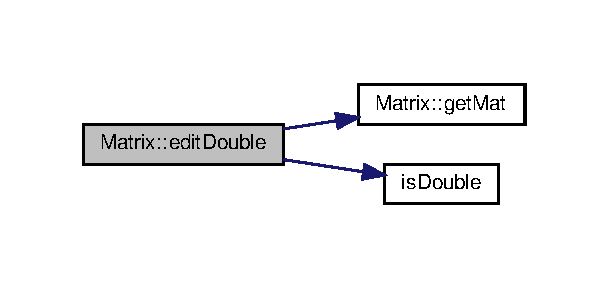
\includegraphics[width=292pt]{class_matrix_a147d3813e96ef757fb0d5ff65e5f97ef_cgraph}
\end{center}
\end{figure}
Here is the caller graph for this function\+:
\nopagebreak
\begin{figure}[H]
\begin{center}
\leavevmode
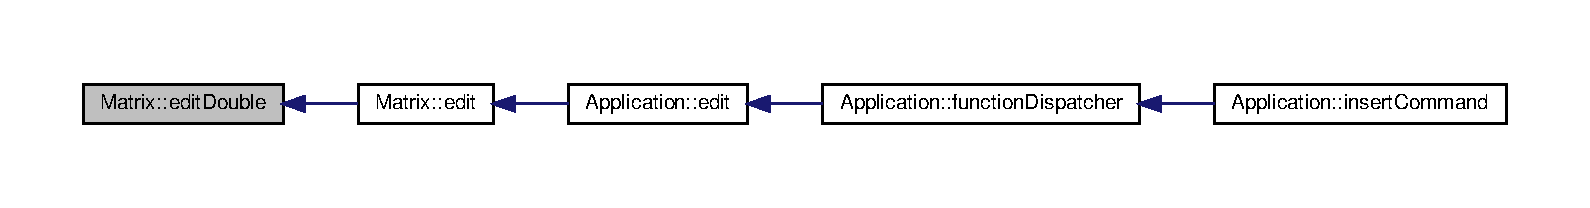
\includegraphics[width=350pt]{class_matrix_a147d3813e96ef757fb0d5ff65e5f97ef_icgraph}
\end{center}
\end{figure}
\mbox{\Hypertarget{class_matrix_af3d26e46fcec1a98380b1af04f008f22}\label{class_matrix_af3d26e46fcec1a98380b1af04f008f22}} 
\index{Matrix@{Matrix}!edit\+Formula@{edit\+Formula}}
\index{edit\+Formula@{edit\+Formula}!Matrix@{Matrix}}
\subsubsection{\texorpdfstring{edit\+Formula()}{editFormula()}}
{\footnotesize\ttfamily \hyperlink{formula_8h_a869e2a5deeb3daa4c82d6bc91cf20d92}{matrix} Matrix\+::edit\+Formula (\begin{DoxyParamCaption}\item[{int}]{row,  }\item[{int}]{col }\end{DoxyParamCaption})\hspace{0.3cm}{\ttfamily [private]}}

Used when editing a cell when the new data type is going to be the result of a formula. 
\begin{DoxyParams}{Parameters}
{\em row} & \\
\hline
{\em col} & \\
\hline
\end{DoxyParams}
Here is the call graph for this function\+:
\nopagebreak
\begin{figure}[H]
\begin{center}
\leavevmode
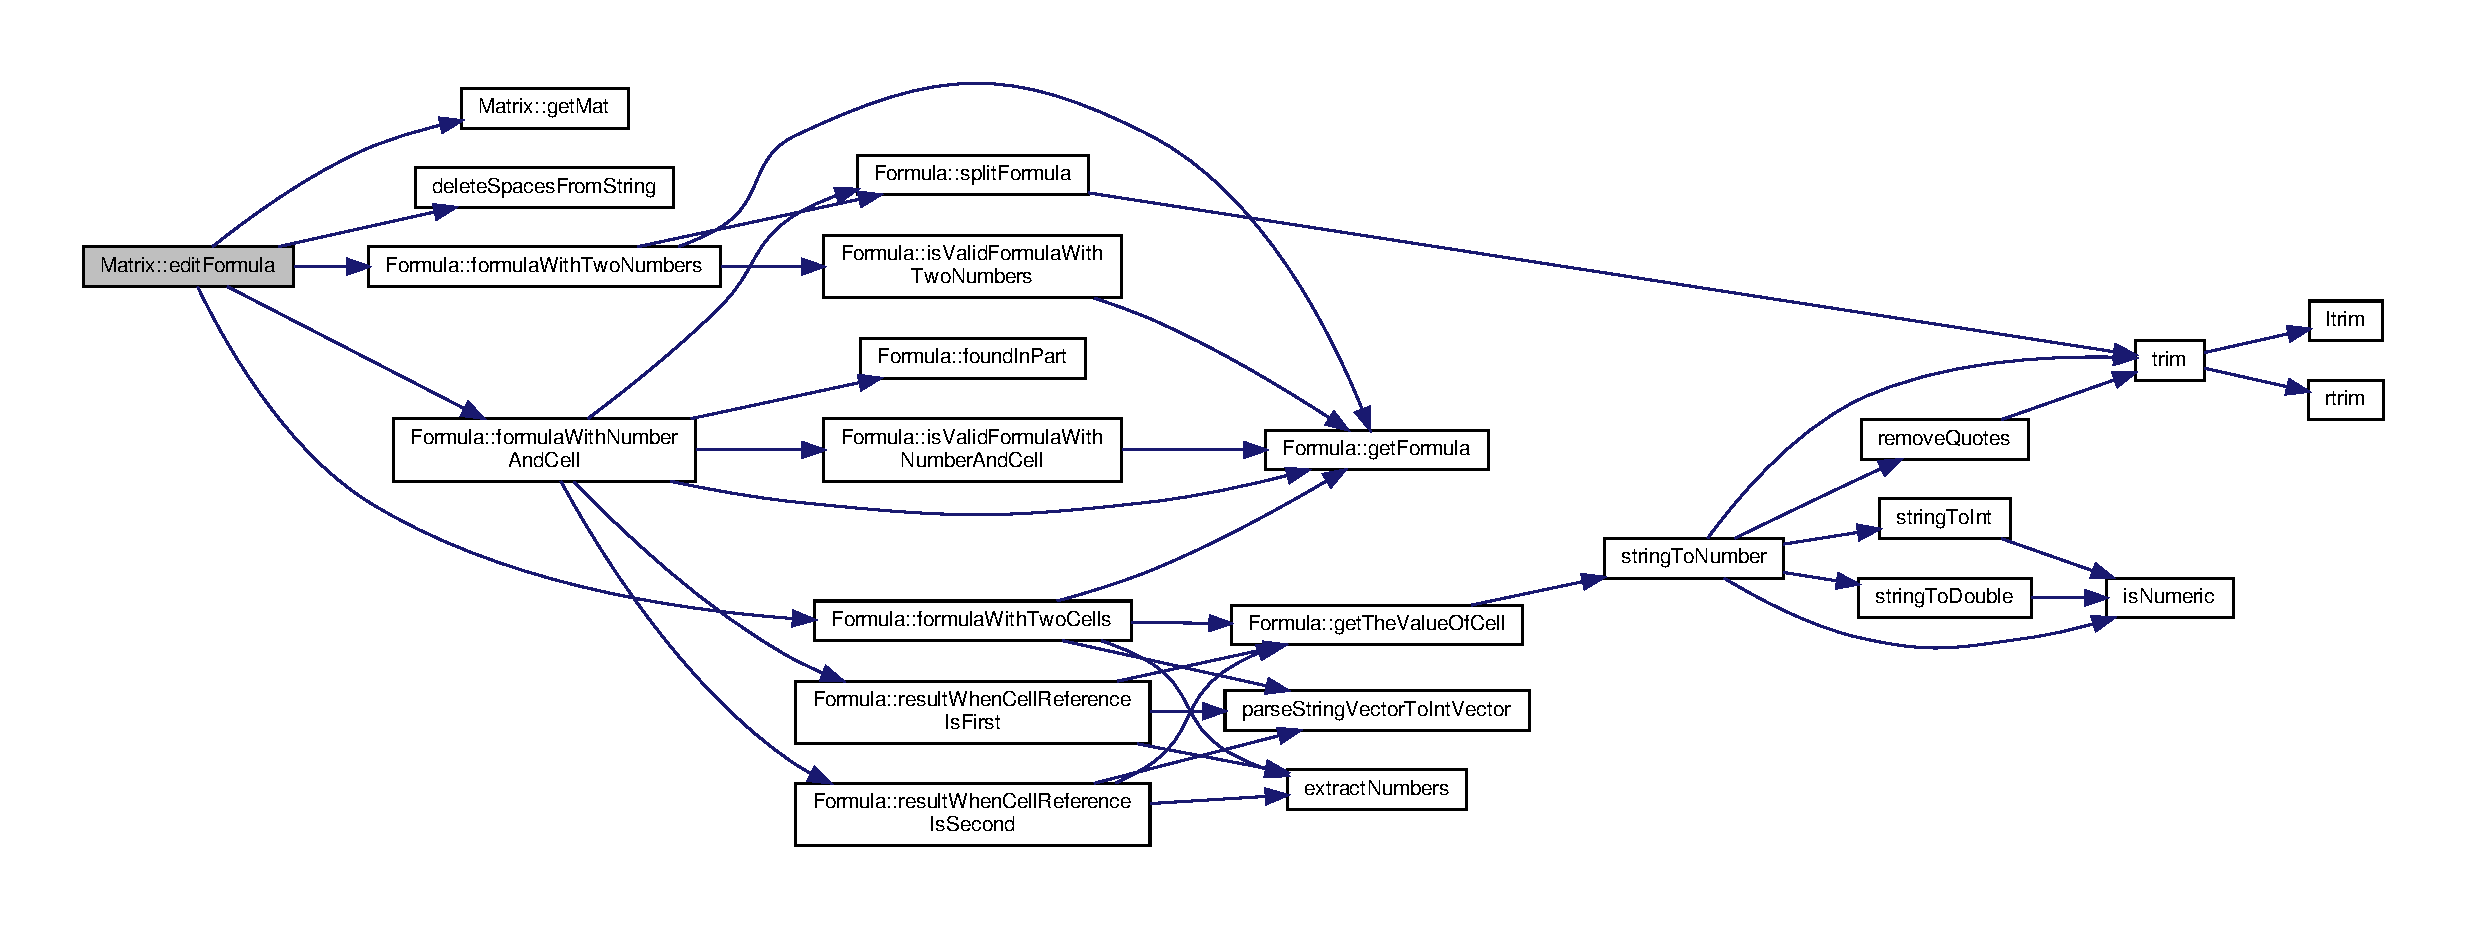
\includegraphics[width=350pt]{class_matrix_af3d26e46fcec1a98380b1af04f008f22_cgraph}
\end{center}
\end{figure}
Here is the caller graph for this function\+:
\nopagebreak
\begin{figure}[H]
\begin{center}
\leavevmode
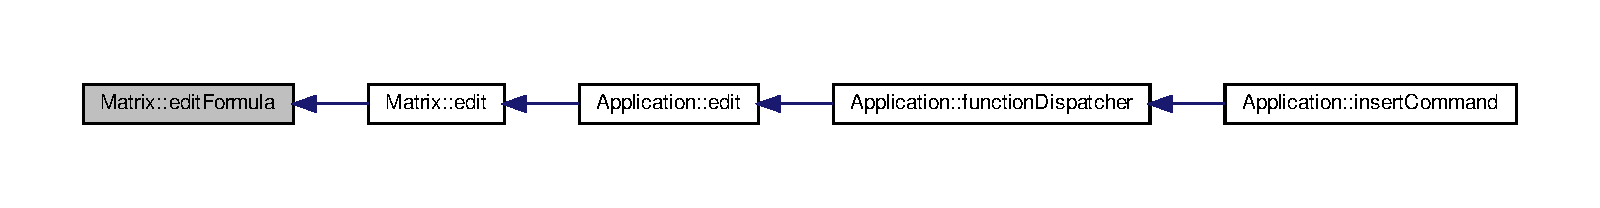
\includegraphics[width=350pt]{class_matrix_af3d26e46fcec1a98380b1af04f008f22_icgraph}
\end{center}
\end{figure}
\mbox{\Hypertarget{class_matrix_a91c66e2961a16adf56b8d58b916d2d46}\label{class_matrix_a91c66e2961a16adf56b8d58b916d2d46}} 
\index{Matrix@{Matrix}!edit\+Integer@{edit\+Integer}}
\index{edit\+Integer@{edit\+Integer}!Matrix@{Matrix}}
\subsubsection{\texorpdfstring{edit\+Integer()}{editInteger()}}
{\footnotesize\ttfamily \hyperlink{formula_8h_a869e2a5deeb3daa4c82d6bc91cf20d92}{matrix} Matrix\+::edit\+Integer (\begin{DoxyParamCaption}\item[{int}]{rol,  }\item[{int}]{col }\end{DoxyParamCaption})\hspace{0.3cm}{\ttfamily [private]}}

Used when editing a cell when the new data type is going to be an integer. 
\begin{DoxyParams}{Parameters}
{\em rol} & \\
\hline
{\em col} & \\
\hline
\end{DoxyParams}
Here is the call graph for this function\+:
\nopagebreak
\begin{figure}[H]
\begin{center}
\leavevmode
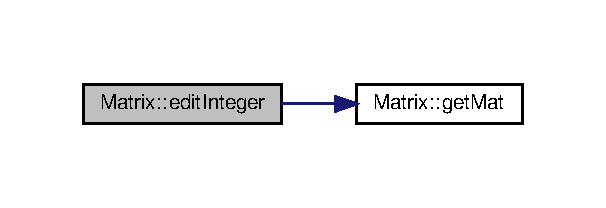
\includegraphics[width=291pt]{class_matrix_a91c66e2961a16adf56b8d58b916d2d46_cgraph}
\end{center}
\end{figure}
Here is the caller graph for this function\+:
\nopagebreak
\begin{figure}[H]
\begin{center}
\leavevmode
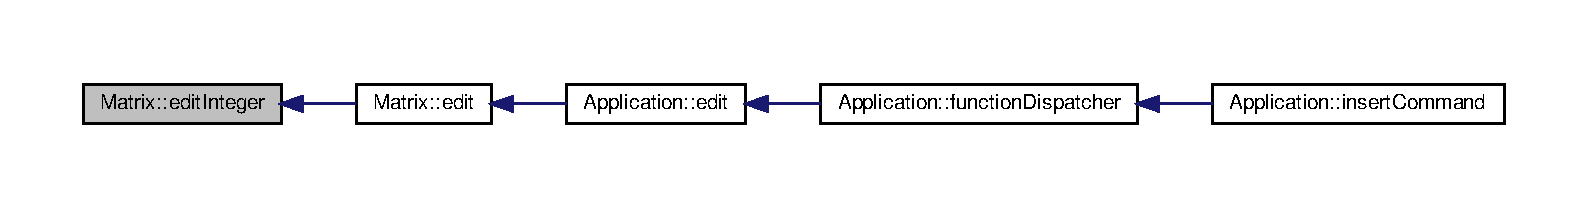
\includegraphics[width=350pt]{class_matrix_a91c66e2961a16adf56b8d58b916d2d46_icgraph}
\end{center}
\end{figure}
\mbox{\Hypertarget{class_matrix_a7029d8a3cd3c691b46adfd777abc880c}\label{class_matrix_a7029d8a3cd3c691b46adfd777abc880c}} 
\index{Matrix@{Matrix}!edit\+String@{edit\+String}}
\index{edit\+String@{edit\+String}!Matrix@{Matrix}}
\subsubsection{\texorpdfstring{edit\+String()}{editString()}}
{\footnotesize\ttfamily \hyperlink{formula_8h_a869e2a5deeb3daa4c82d6bc91cf20d92}{matrix} Matrix\+::edit\+String (\begin{DoxyParamCaption}\item[{int}]{rol,  }\item[{int}]{col }\end{DoxyParamCaption})\hspace{0.3cm}{\ttfamily [private]}}

Used when editing a cell when the new data type is going to be a string. 
\begin{DoxyParams}{Parameters}
{\em rol} & \\
\hline
{\em col} & \\
\hline
\end{DoxyParams}
Here is the call graph for this function\+:
\nopagebreak
\begin{figure}[H]
\begin{center}
\leavevmode
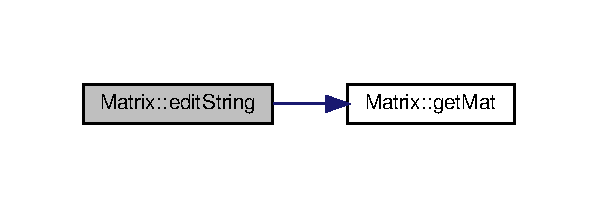
\includegraphics[width=287pt]{class_matrix_a7029d8a3cd3c691b46adfd777abc880c_cgraph}
\end{center}
\end{figure}
Here is the caller graph for this function\+:
\nopagebreak
\begin{figure}[H]
\begin{center}
\leavevmode
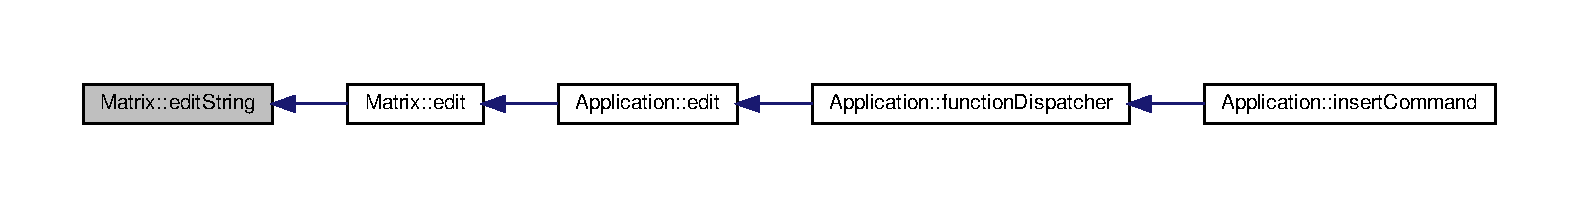
\includegraphics[width=350pt]{class_matrix_a7029d8a3cd3c691b46adfd777abc880c_icgraph}
\end{center}
\end{figure}
\mbox{\Hypertarget{class_matrix_a35eb9dcb01c552fea1f5926db35339ef}\label{class_matrix_a35eb9dcb01c552fea1f5926db35339ef}} 
\index{Matrix@{Matrix}!file\+To\+Matrix@{file\+To\+Matrix}}
\index{file\+To\+Matrix@{file\+To\+Matrix}!Matrix@{Matrix}}
\subsubsection{\texorpdfstring{file\+To\+Matrix()}{fileToMatrix()}}
{\footnotesize\ttfamily \hyperlink{formula_8h_a869e2a5deeb3daa4c82d6bc91cf20d92}{matrix} Matrix\+::file\+To\+Matrix (\begin{DoxyParamCaption}\item[{const string \&}]{filename }\end{DoxyParamCaption})}

Method that is reading the information from a file and saves it into a matrix. 
\begin{DoxyParams}{Parameters}
{\em filename} & \\
\hline
\end{DoxyParams}
\begin{DoxyReturn}{Returns}
matrix 
\end{DoxyReturn}
Here is the caller graph for this function\+:
\nopagebreak
\begin{figure}[H]
\begin{center}
\leavevmode
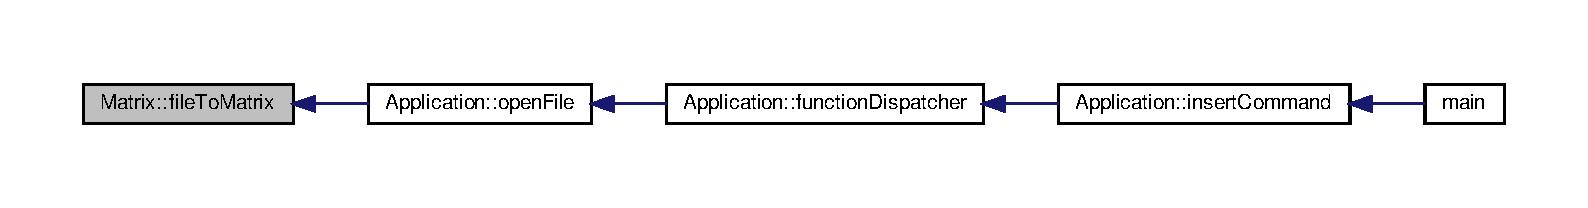
\includegraphics[width=350pt]{class_matrix_a35eb9dcb01c552fea1f5926db35339ef_icgraph}
\end{center}
\end{figure}
\mbox{\Hypertarget{class_matrix_a0c8e09a50ddb4d068d39456ea130abcc}\label{class_matrix_a0c8e09a50ddb4d068d39456ea130abcc}} 
\index{Matrix@{Matrix}!get\+Instance@{get\+Instance}}
\index{get\+Instance@{get\+Instance}!Matrix@{Matrix}}
\subsubsection{\texorpdfstring{get\+Instance()}{getInstance()}}
{\footnotesize\ttfamily static \hyperlink{class_matrix}{Matrix}$\ast$ Matrix\+::get\+Instance (\begin{DoxyParamCaption}{ }\end{DoxyParamCaption})\hspace{0.3cm}{\ttfamily [inline]}, {\ttfamily [static]}}

Method that servers as a constructor but it does not initialize a new object. It is accessing the same instance of this class over and over. Here is the caller graph for this function\+:
\nopagebreak
\begin{figure}[H]
\begin{center}
\leavevmode
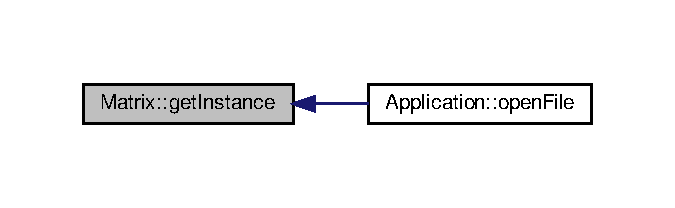
\includegraphics[width=350pt]{class_matrix_a0c8e09a50ddb4d068d39456ea130abcc_icgraph}
\end{center}
\end{figure}
\mbox{\Hypertarget{class_matrix_a52d82641f52304c9b6525747cd7f960c}\label{class_matrix_a52d82641f52304c9b6525747cd7f960c}} 
\index{Matrix@{Matrix}!get\+Mat@{get\+Mat}}
\index{get\+Mat@{get\+Mat}!Matrix@{Matrix}}
\subsubsection{\texorpdfstring{get\+Mat()}{getMat()}}
{\footnotesize\ttfamily const \hyperlink{formula_8h_a869e2a5deeb3daa4c82d6bc91cf20d92}{matrix} \& Matrix\+::get\+Mat (\begin{DoxyParamCaption}{ }\end{DoxyParamCaption}) const}

Getter for matrix. \begin{DoxyReturn}{Returns}
matrix 
\end{DoxyReturn}
Here is the caller graph for this function\+:
\nopagebreak
\begin{figure}[H]
\begin{center}
\leavevmode
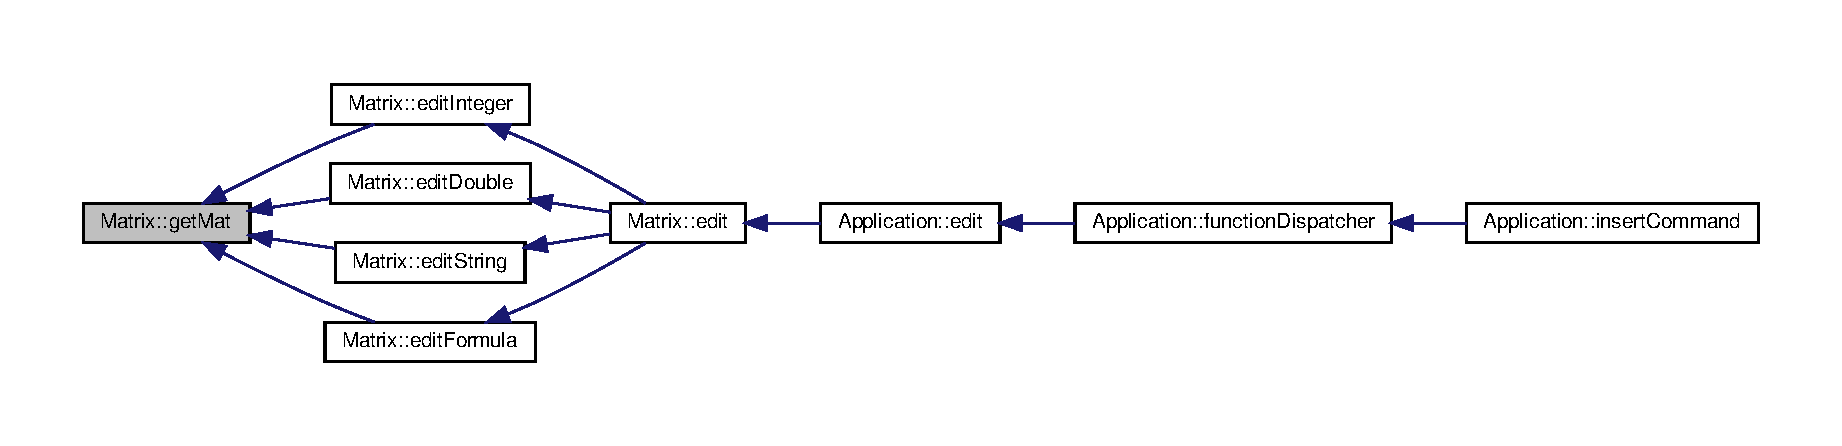
\includegraphics[width=350pt]{class_matrix_a52d82641f52304c9b6525747cd7f960c_icgraph}
\end{center}
\end{figure}
\mbox{\Hypertarget{class_matrix_a8620c5426a31cf8fe0072df32bb3f65d}\label{class_matrix_a8620c5426a31cf8fe0072df32bb3f65d}} 
\index{Matrix@{Matrix}!max\+Element\+Per\+Row\+Whole\+Table@{max\+Element\+Per\+Row\+Whole\+Table}}
\index{max\+Element\+Per\+Row\+Whole\+Table@{max\+Element\+Per\+Row\+Whole\+Table}!Matrix@{Matrix}}
\subsubsection{\texorpdfstring{max\+Element\+Per\+Row\+Whole\+Table()}{maxElementPerRowWholeTable()}}
{\footnotesize\ttfamily int Matrix\+::max\+Element\+Per\+Row\+Whole\+Table (\begin{DoxyParamCaption}{ }\end{DoxyParamCaption})\hspace{0.3cm}{\ttfamily [private]}}

Method returns the number of elements on the row with the most elements. \begin{DoxyReturn}{Returns}
int 
\end{DoxyReturn}
Here is the caller graph for this function\+:
\nopagebreak
\begin{figure}[H]
\begin{center}
\leavevmode
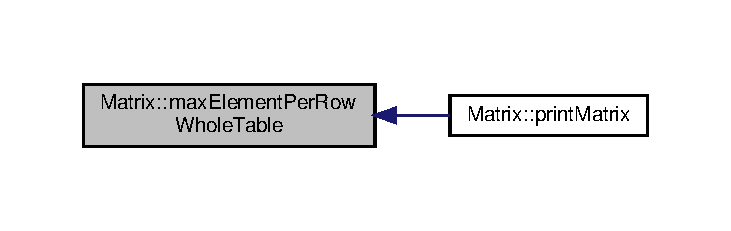
\includegraphics[width=350pt]{class_matrix_a8620c5426a31cf8fe0072df32bb3f65d_icgraph}
\end{center}
\end{figure}
\mbox{\Hypertarget{class_matrix_a60dac9b70e73a12d2adb32d6be9ff65d}\label{class_matrix_a60dac9b70e73a12d2adb32d6be9ff65d}} 
\index{Matrix@{Matrix}!max\+Width\+Of\+Cell@{max\+Width\+Of\+Cell}}
\index{max\+Width\+Of\+Cell@{max\+Width\+Of\+Cell}!Matrix@{Matrix}}
\subsubsection{\texorpdfstring{max\+Width\+Of\+Cell()}{maxWidthOfCell()}}
{\footnotesize\ttfamily int Matrix\+::max\+Width\+Of\+Cell (\begin{DoxyParamCaption}{ }\end{DoxyParamCaption})\hspace{0.3cm}{\ttfamily [private]}}

Returns the length of the longest cell in the table. \begin{DoxyReturn}{Returns}
int 
\end{DoxyReturn}
Here is the caller graph for this function\+:
\nopagebreak
\begin{figure}[H]
\begin{center}
\leavevmode
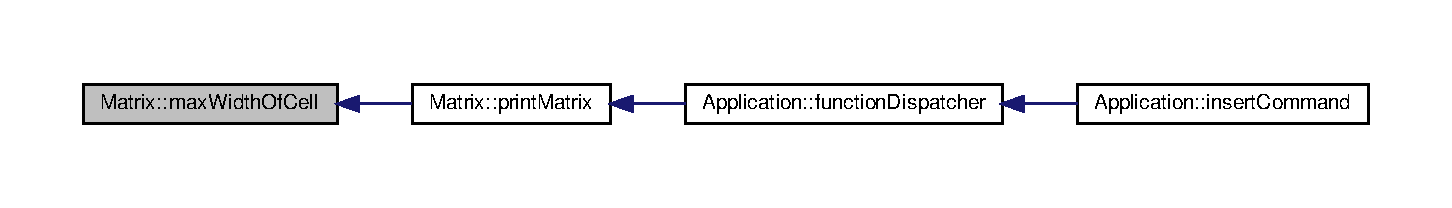
\includegraphics[width=350pt]{class_matrix_a60dac9b70e73a12d2adb32d6be9ff65d_icgraph}
\end{center}
\end{figure}
\mbox{\Hypertarget{class_matrix_aa1967ad240a5ffaf492800044b7275d9}\label{class_matrix_aa1967ad240a5ffaf492800044b7275d9}} 
\index{Matrix@{Matrix}!print\+Matrix@{print\+Matrix}}
\index{print\+Matrix@{print\+Matrix}!Matrix@{Matrix}}
\subsubsection{\texorpdfstring{print\+Matrix()}{printMatrix()}}
{\footnotesize\ttfamily void Matrix\+::print\+Matrix (\begin{DoxyParamCaption}{ }\end{DoxyParamCaption})}

Method displaying the matrix. Here is the call graph for this function\+:
\nopagebreak
\begin{figure}[H]
\begin{center}
\leavevmode
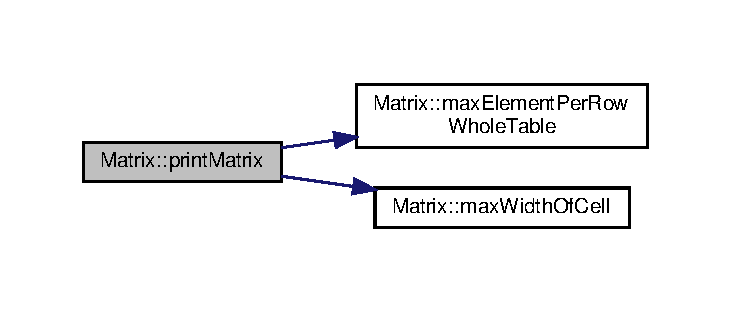
\includegraphics[width=350pt]{class_matrix_aa1967ad240a5ffaf492800044b7275d9_cgraph}
\end{center}
\end{figure}
Here is the caller graph for this function\+:
\nopagebreak
\begin{figure}[H]
\begin{center}
\leavevmode
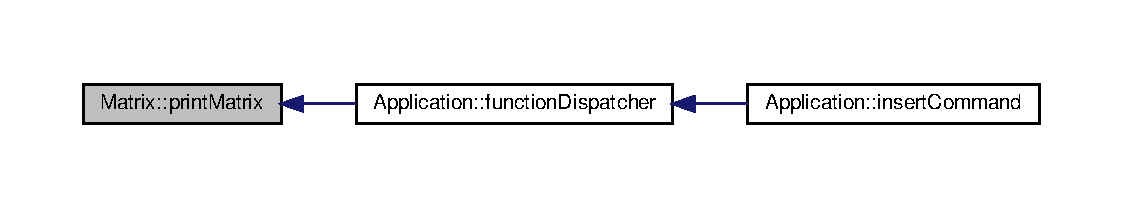
\includegraphics[width=350pt]{class_matrix_aa1967ad240a5ffaf492800044b7275d9_icgraph}
\end{center}
\end{figure}
\mbox{\Hypertarget{class_matrix_a8c45dd1354fa25e14065cab23f3074c0}\label{class_matrix_a8c45dd1354fa25e14065cab23f3074c0}} 
\index{Matrix@{Matrix}!set\+Matrix@{set\+Matrix}}
\index{set\+Matrix@{set\+Matrix}!Matrix@{Matrix}}
\subsubsection{\texorpdfstring{set\+Matrix()}{setMatrix()}}
{\footnotesize\ttfamily void Matrix\+::set\+Matrix (\begin{DoxyParamCaption}\item[{const \hyperlink{formula_8h_a869e2a5deeb3daa4c82d6bc91cf20d92}{matrix} \&}]{mat }\end{DoxyParamCaption})\hspace{0.3cm}{\ttfamily [inline]}}

Method setting a matrix. 
\begin{DoxyParams}{Parameters}
{\em mat} & \\
\hline
\end{DoxyParams}
Here is the caller graph for this function\+:
\nopagebreak
\begin{figure}[H]
\begin{center}
\leavevmode
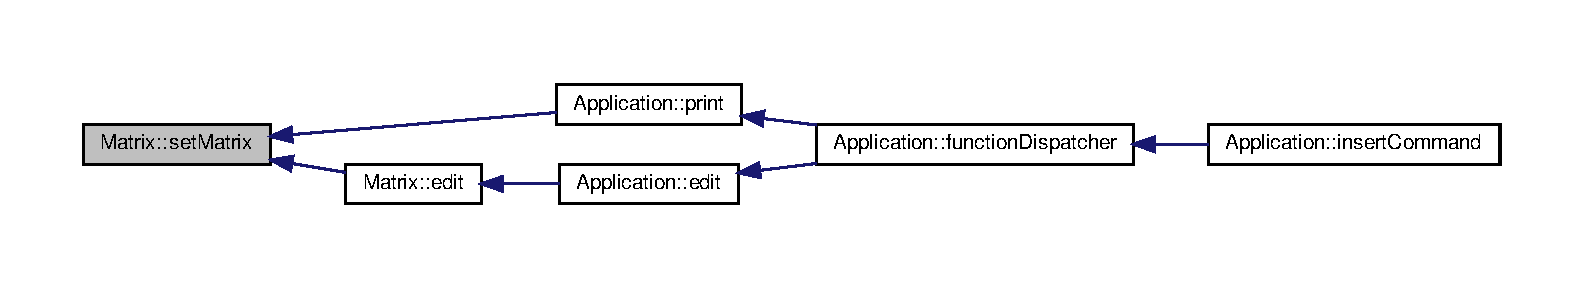
\includegraphics[width=350pt]{class_matrix_a8c45dd1354fa25e14065cab23f3074c0_icgraph}
\end{center}
\end{figure}


\subsection{Member Data Documentation}
\mbox{\Hypertarget{class_matrix_adbe13eefa6a6ea2f02f45da26400f22e}\label{class_matrix_adbe13eefa6a6ea2f02f45da26400f22e}} 
\index{Matrix@{Matrix}!instance@{instance}}
\index{instance@{instance}!Matrix@{Matrix}}
\subsubsection{\texorpdfstring{instance}{instance}}
{\footnotesize\ttfamily \hyperlink{class_matrix}{Matrix} $\ast$ Matrix\+::instance = 0\hspace{0.3cm}{\ttfamily [static]}, {\ttfamily [private]}}

\mbox{\Hypertarget{class_matrix_a1b0c75c45092426431308172aab92c66}\label{class_matrix_a1b0c75c45092426431308172aab92c66}} 
\index{Matrix@{Matrix}!mat@{mat}}
\index{mat@{mat}!Matrix@{Matrix}}
\subsubsection{\texorpdfstring{mat}{mat}}
{\footnotesize\ttfamily \hyperlink{formula_8h_a869e2a5deeb3daa4c82d6bc91cf20d92}{matrix} Matrix\+::mat\hspace{0.3cm}{\ttfamily [private]}}



The documentation for this class was generated from the following files\+:\begin{DoxyCompactItemize}
\item 
\hyperlink{matrix_8h}{matrix.\+h}\item 
\hyperlink{matrix_8cpp}{matrix.\+cpp}\end{DoxyCompactItemize}

\chapter{File Documentation}
\hypertarget{string_utils_8h}{}\section{string\+Utils.\+h File Reference}
\label{string_utils_8h}\index{string\+Utils.\+h@{string\+Utils.\+h}}


String modifiers.  


{\ttfamily \#include $<$string$>$}\newline
{\ttfamily \#include $<$sstream$>$}\newline
Include dependency graph for string\+Utils.\+h\+:\nopagebreak
\begin{figure}[H]
\begin{center}
\leavevmode
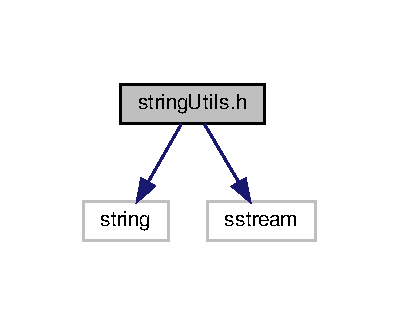
\includegraphics[width=192pt]{string_utils_8h__incl}
\end{center}
\end{figure}
\subsection*{Functions}
\begin{DoxyCompactItemize}
\item 
bool \hyperlink{string_utils_8h_a9d52b2e7847c950eee6a01ae597679fa}{is\+Numeric} (const string \&str)
\item 
int \hyperlink{string_utils_8h_a2ba9357b7f0235a408b4c3fd26526b2d}{string\+To\+Int} (const string \&number\+String)
\item 
double \hyperlink{string_utils_8h_a5e388b01a5a212fa4f231ea35efa3a78}{string\+To\+Double} (const string \&number\+String)
\item 
string \& \hyperlink{string_utils_8h_a92e1949f46533a5674ce0cc6d3350b95}{ltrim} (string \&str)
\item 
string \& \hyperlink{string_utils_8h_ac869ec7686a817321f7f80556f5b2bfb}{rtrim} (string \&str)
\item 
string \& \hyperlink{string_utils_8h_af941fe852e0b5d8235ddc3296b8b00d3}{trim} (string \&str)
\item 
void \hyperlink{string_utils_8h_ae79bd017557b754bb1ff0e42a824ffc5}{remove\+Quotes} (string \&str)
\item 
double \hyperlink{string_utils_8h_a0e10b75736c375cf8a40f59579871ef1}{string\+To\+Number} (string number\+String)
\item 
void \hyperlink{string_utils_8h_aaa9610e8d77442d8f5cb10a5b77666da}{extract\+Numbers} (vector$<$ string $>$ \&rows\+Cols, const string \&str)
\item 
vector$<$ int $>$ \hyperlink{string_utils_8h_ae302876f17c45ff94972bafa8580a3b8}{parse\+String\+Vector\+To\+Int\+Vector} (const vector$<$ string $>$ \&rows\+Cols)
\end{DoxyCompactItemize}


\subsection{Detailed Description}
String modifiers. 



\subsection{Function Documentation}
\mbox{\Hypertarget{string_utils_8h_aaa9610e8d77442d8f5cb10a5b77666da}\label{string_utils_8h_aaa9610e8d77442d8f5cb10a5b77666da}} 
\index{string\+Utils.\+h@{string\+Utils.\+h}!extract\+Numbers@{extract\+Numbers}}
\index{extract\+Numbers@{extract\+Numbers}!string\+Utils.\+h@{string\+Utils.\+h}}
\subsubsection{\texorpdfstring{extract\+Numbers()}{extractNumbers()}}
{\footnotesize\ttfamily void extract\+Numbers (\begin{DoxyParamCaption}\item[{vector$<$ string $>$ \&}]{rows\+Cols,  }\item[{const string \&}]{str }\end{DoxyParamCaption})}

Uses regular expression to extract all the coordinates from a reference to a cell. 
\begin{DoxyParams}{Parameters}
{\em rows\+Cols} & \\
\hline
{\em str} & \\
\hline
\end{DoxyParams}
Here is the caller graph for this function\+:
\nopagebreak
\begin{figure}[H]
\begin{center}
\leavevmode
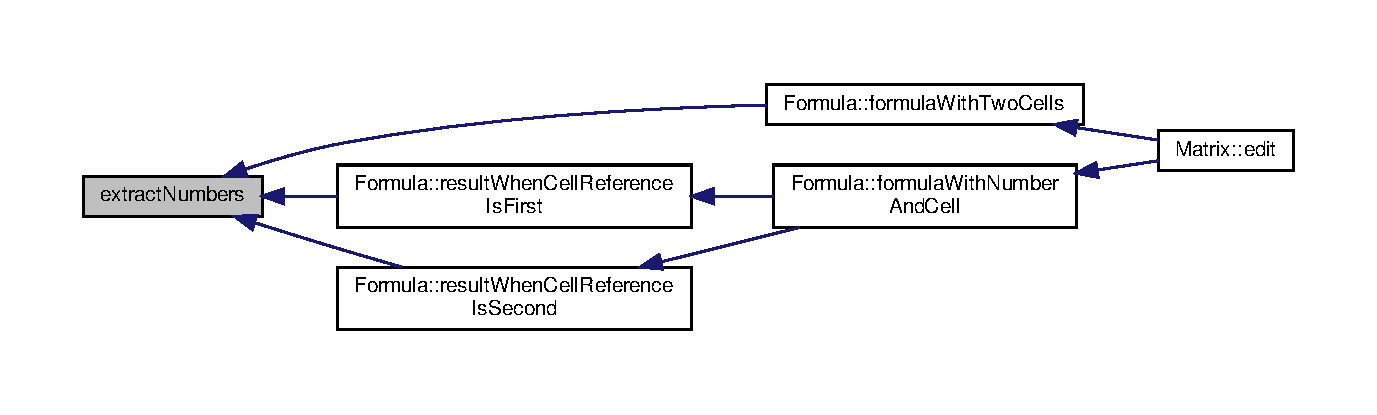
\includegraphics[width=350pt]{string_utils_8h_aaa9610e8d77442d8f5cb10a5b77666da_icgraph}
\end{center}
\end{figure}
\mbox{\Hypertarget{string_utils_8h_a9d52b2e7847c950eee6a01ae597679fa}\label{string_utils_8h_a9d52b2e7847c950eee6a01ae597679fa}} 
\index{string\+Utils.\+h@{string\+Utils.\+h}!is\+Numeric@{is\+Numeric}}
\index{is\+Numeric@{is\+Numeric}!string\+Utils.\+h@{string\+Utils.\+h}}
\subsubsection{\texorpdfstring{is\+Numeric()}{isNumeric()}}
{\footnotesize\ttfamily bool is\+Numeric (\begin{DoxyParamCaption}\item[{const string \&}]{str }\end{DoxyParamCaption})}

Does the string str contains only numeric symbols. 
\begin{DoxyParams}{Parameters}
{\em string} & \\
\hline
\end{DoxyParams}
\begin{DoxyReturn}{Returns}
true or false 
\end{DoxyReturn}
Here is the caller graph for this function\+:
\nopagebreak
\begin{figure}[H]
\begin{center}
\leavevmode
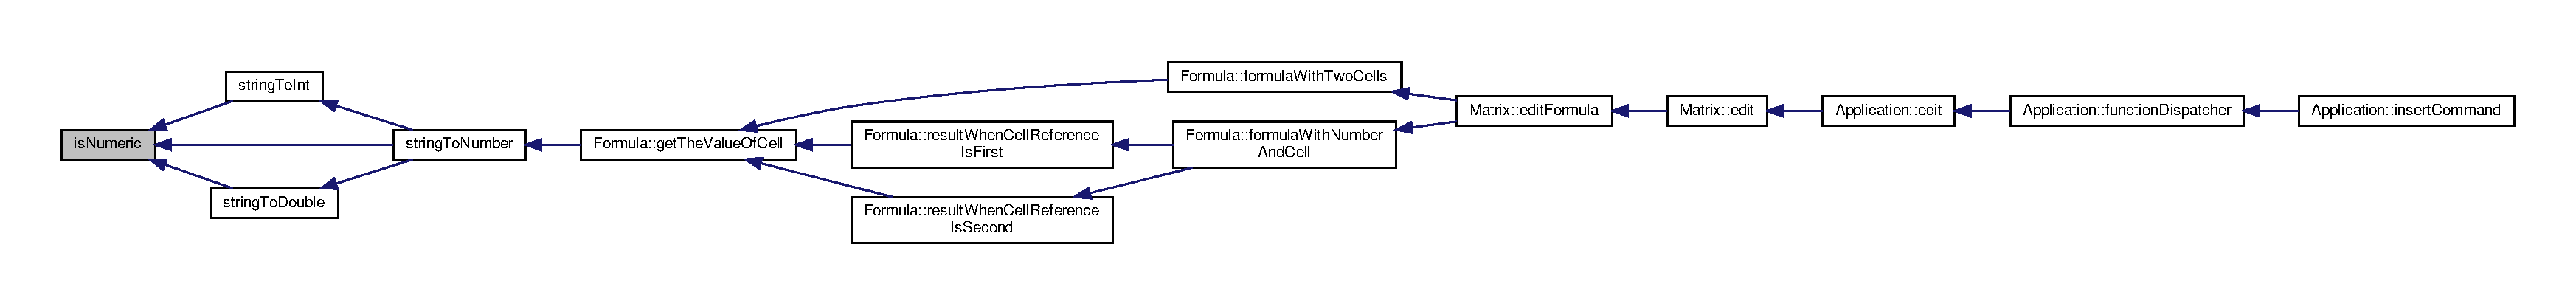
\includegraphics[width=350pt]{string_utils_8h_a9d52b2e7847c950eee6a01ae597679fa_icgraph}
\end{center}
\end{figure}
\mbox{\Hypertarget{string_utils_8h_a92e1949f46533a5674ce0cc6d3350b95}\label{string_utils_8h_a92e1949f46533a5674ce0cc6d3350b95}} 
\index{string\+Utils.\+h@{string\+Utils.\+h}!ltrim@{ltrim}}
\index{ltrim@{ltrim}!string\+Utils.\+h@{string\+Utils.\+h}}
\subsubsection{\texorpdfstring{ltrim()}{ltrim()}}
{\footnotesize\ttfamily string \& ltrim (\begin{DoxyParamCaption}\item[{string \&}]{str }\end{DoxyParamCaption})}

Removes the whitespaces from the left side of the string. 
\begin{DoxyParams}{Parameters}
{\em string} & \\
\hline
\end{DoxyParams}
\begin{DoxyReturn}{Returns}
string 
\end{DoxyReturn}
Here is the caller graph for this function\+:
\nopagebreak
\begin{figure}[H]
\begin{center}
\leavevmode
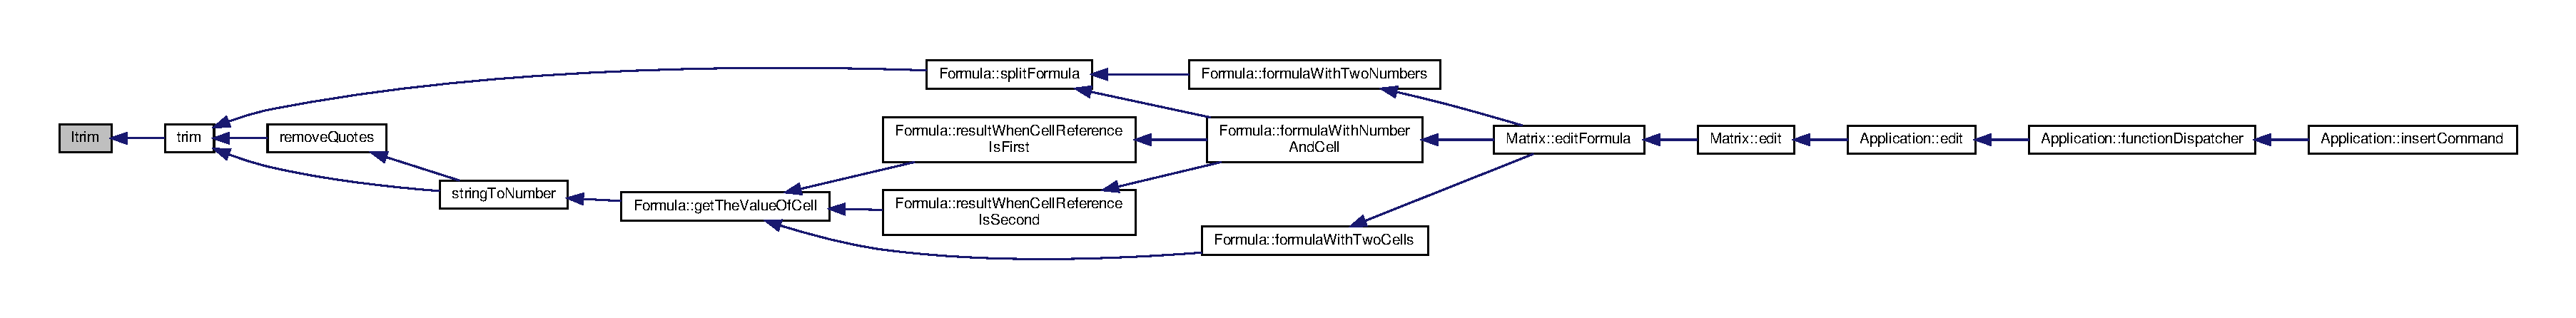
\includegraphics[width=350pt]{string_utils_8h_a92e1949f46533a5674ce0cc6d3350b95_icgraph}
\end{center}
\end{figure}
\mbox{\Hypertarget{string_utils_8h_ae302876f17c45ff94972bafa8580a3b8}\label{string_utils_8h_ae302876f17c45ff94972bafa8580a3b8}} 
\index{string\+Utils.\+h@{string\+Utils.\+h}!parse\+String\+Vector\+To\+Int\+Vector@{parse\+String\+Vector\+To\+Int\+Vector}}
\index{parse\+String\+Vector\+To\+Int\+Vector@{parse\+String\+Vector\+To\+Int\+Vector}!string\+Utils.\+h@{string\+Utils.\+h}}
\subsubsection{\texorpdfstring{parse\+String\+Vector\+To\+Int\+Vector()}{parseStringVectorToIntVector()}}
{\footnotesize\ttfamily vector$<$int$>$ parse\+String\+Vector\+To\+Int\+Vector (\begin{DoxyParamCaption}\item[{const vector$<$ string $>$ \&}]{rows\+Cols }\end{DoxyParamCaption})}

Accepting vector$<$string$>$ and returns vector$<$int$>$. 
\begin{DoxyParams}{Parameters}
{\em vector$<$string$>$} & rows\+Cols \\
\hline
\end{DoxyParams}
\begin{DoxyReturn}{Returns}
vector$<$int$>$ 
\end{DoxyReturn}
Here is the caller graph for this function\+:
\nopagebreak
\begin{figure}[H]
\begin{center}
\leavevmode
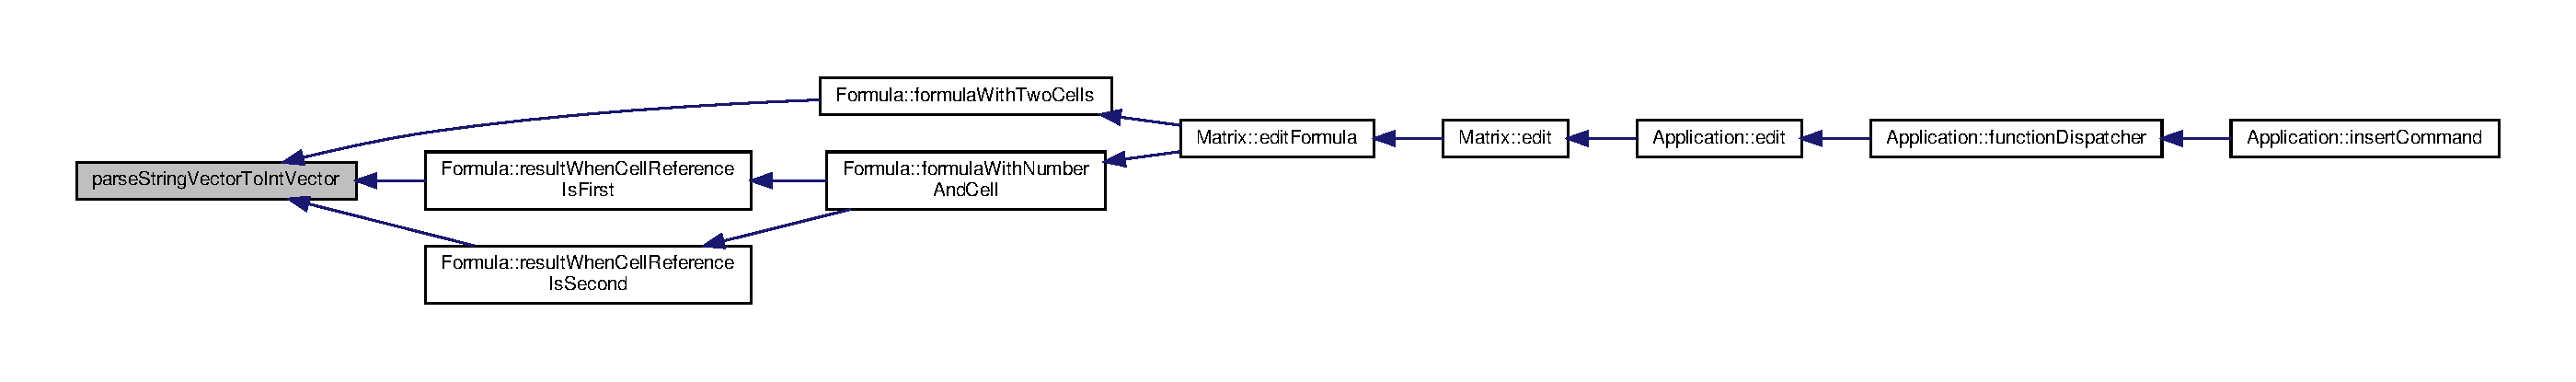
\includegraphics[width=350pt]{string_utils_8h_ae302876f17c45ff94972bafa8580a3b8_icgraph}
\end{center}
\end{figure}
\mbox{\Hypertarget{string_utils_8h_ae79bd017557b754bb1ff0e42a824ffc5}\label{string_utils_8h_ae79bd017557b754bb1ff0e42a824ffc5}} 
\index{string\+Utils.\+h@{string\+Utils.\+h}!remove\+Quotes@{remove\+Quotes}}
\index{remove\+Quotes@{remove\+Quotes}!string\+Utils.\+h@{string\+Utils.\+h}}
\subsubsection{\texorpdfstring{remove\+Quotes()}{removeQuotes()}}
{\footnotesize\ttfamily void remove\+Quotes (\begin{DoxyParamCaption}\item[{string \&}]{str }\end{DoxyParamCaption})}

Remove the quotes from a string. 
\begin{DoxyParams}{Parameters}
{\em str} & \\
\hline
\end{DoxyParams}
Here is the call graph for this function\+:
\nopagebreak
\begin{figure}[H]
\begin{center}
\leavevmode
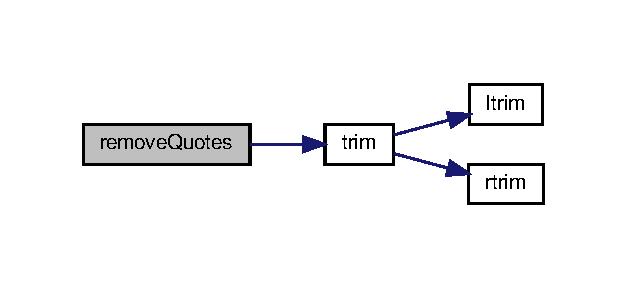
\includegraphics[width=301pt]{string_utils_8h_ae79bd017557b754bb1ff0e42a824ffc5_cgraph}
\end{center}
\end{figure}
Here is the caller graph for this function\+:
\nopagebreak
\begin{figure}[H]
\begin{center}
\leavevmode
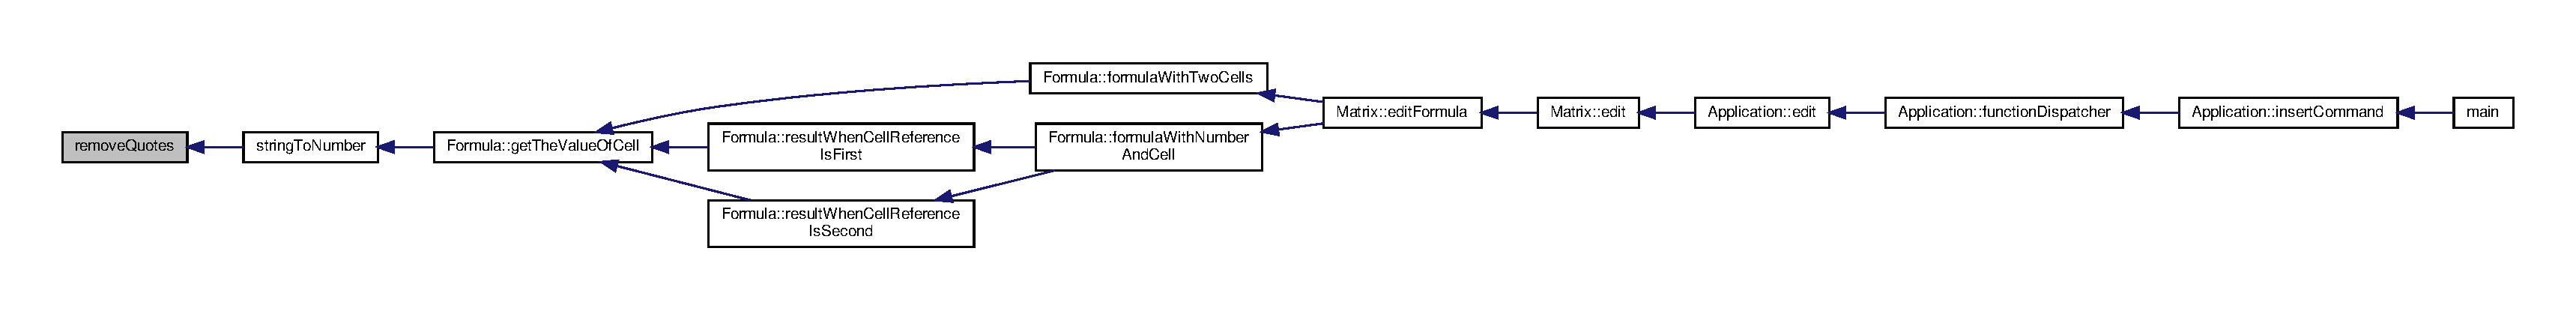
\includegraphics[width=350pt]{string_utils_8h_ae79bd017557b754bb1ff0e42a824ffc5_icgraph}
\end{center}
\end{figure}
\mbox{\Hypertarget{string_utils_8h_ac869ec7686a817321f7f80556f5b2bfb}\label{string_utils_8h_ac869ec7686a817321f7f80556f5b2bfb}} 
\index{string\+Utils.\+h@{string\+Utils.\+h}!rtrim@{rtrim}}
\index{rtrim@{rtrim}!string\+Utils.\+h@{string\+Utils.\+h}}
\subsubsection{\texorpdfstring{rtrim()}{rtrim()}}
{\footnotesize\ttfamily string \& rtrim (\begin{DoxyParamCaption}\item[{string \&}]{str }\end{DoxyParamCaption})}

Removes the whitespaces from the right side of the string. 
\begin{DoxyParams}{Parameters}
{\em string} & \\
\hline
\end{DoxyParams}
\begin{DoxyReturn}{Returns}
string 
\end{DoxyReturn}
Here is the caller graph for this function\+:
\nopagebreak
\begin{figure}[H]
\begin{center}
\leavevmode
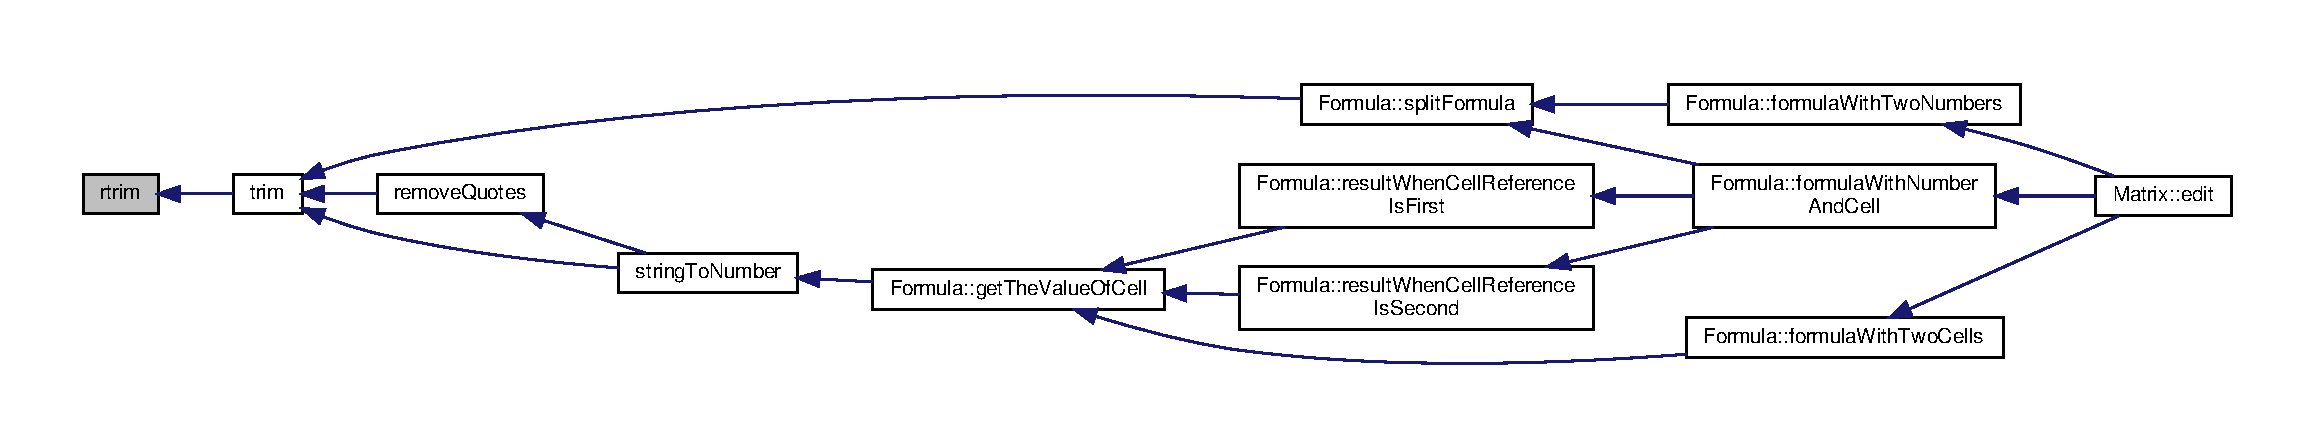
\includegraphics[width=350pt]{string_utils_8h_ac869ec7686a817321f7f80556f5b2bfb_icgraph}
\end{center}
\end{figure}
\mbox{\Hypertarget{string_utils_8h_a5e388b01a5a212fa4f231ea35efa3a78}\label{string_utils_8h_a5e388b01a5a212fa4f231ea35efa3a78}} 
\index{string\+Utils.\+h@{string\+Utils.\+h}!string\+To\+Double@{string\+To\+Double}}
\index{string\+To\+Double@{string\+To\+Double}!string\+Utils.\+h@{string\+Utils.\+h}}
\subsubsection{\texorpdfstring{string\+To\+Double()}{stringToDouble()}}
{\footnotesize\ttfamily double string\+To\+Double (\begin{DoxyParamCaption}\item[{const string \&}]{number\+String }\end{DoxyParamCaption})}

Parsing type string to type double. 
\begin{DoxyParams}{Parameters}
{\em number\+String} & \\
\hline
\end{DoxyParams}
\begin{DoxyReturn}{Returns}
result\+Double 
\end{DoxyReturn}
Here is the call graph for this function\+:
\nopagebreak
\begin{figure}[H]
\begin{center}
\leavevmode
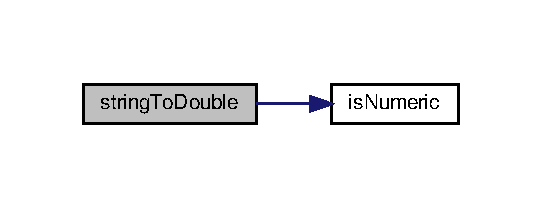
\includegraphics[width=260pt]{string_utils_8h_a5e388b01a5a212fa4f231ea35efa3a78_cgraph}
\end{center}
\end{figure}
Here is the caller graph for this function\+:
\nopagebreak
\begin{figure}[H]
\begin{center}
\leavevmode
\includegraphics[width=350pt]{string_utils_8h_a5e388b01a5a212fa4f231ea35efa3a78_icgraph}
\end{center}
\end{figure}
\mbox{\Hypertarget{string_utils_8h_a2ba9357b7f0235a408b4c3fd26526b2d}\label{string_utils_8h_a2ba9357b7f0235a408b4c3fd26526b2d}} 
\index{string\+Utils.\+h@{string\+Utils.\+h}!string\+To\+Int@{string\+To\+Int}}
\index{string\+To\+Int@{string\+To\+Int}!string\+Utils.\+h@{string\+Utils.\+h}}
\subsubsection{\texorpdfstring{string\+To\+Int()}{stringToInt()}}
{\footnotesize\ttfamily int string\+To\+Int (\begin{DoxyParamCaption}\item[{const string \&}]{number\+String }\end{DoxyParamCaption})}

Parsing type string to type int. 
\begin{DoxyParams}{Parameters}
{\em number\+String} & \\
\hline
\end{DoxyParams}
\begin{DoxyReturn}{Returns}
result\+Int 
\end{DoxyReturn}
Here is the call graph for this function\+:
\nopagebreak
\begin{figure}[H]
\begin{center}
\leavevmode
\includegraphics[width=240pt]{string_utils_8h_a2ba9357b7f0235a408b4c3fd26526b2d_cgraph}
\end{center}
\end{figure}
Here is the caller graph for this function\+:
\nopagebreak
\begin{figure}[H]
\begin{center}
\leavevmode
\includegraphics[width=350pt]{string_utils_8h_a2ba9357b7f0235a408b4c3fd26526b2d_icgraph}
\end{center}
\end{figure}
\mbox{\Hypertarget{string_utils_8h_a0e10b75736c375cf8a40f59579871ef1}\label{string_utils_8h_a0e10b75736c375cf8a40f59579871ef1}} 
\index{string\+Utils.\+h@{string\+Utils.\+h}!string\+To\+Number@{string\+To\+Number}}
\index{string\+To\+Number@{string\+To\+Number}!string\+Utils.\+h@{string\+Utils.\+h}}
\subsubsection{\texorpdfstring{string\+To\+Number()}{stringToNumber()}}
{\footnotesize\ttfamily double string\+To\+Number (\begin{DoxyParamCaption}\item[{string}]{number\+String }\end{DoxyParamCaption})}

Parse a string to a number. 
\begin{DoxyParams}{Parameters}
{\em number\+String} & \\
\hline
\end{DoxyParams}
\begin{DoxyReturn}{Returns}

\end{DoxyReturn}
Here is the call graph for this function\+:
\nopagebreak
\begin{figure}[H]
\begin{center}
\leavevmode
\includegraphics[width=350pt]{string_utils_8h_a0e10b75736c375cf8a40f59579871ef1_cgraph}
\end{center}
\end{figure}
Here is the caller graph for this function\+:
\nopagebreak
\begin{figure}[H]
\begin{center}
\leavevmode
\includegraphics[width=350pt]{string_utils_8h_a0e10b75736c375cf8a40f59579871ef1_icgraph}
\end{center}
\end{figure}
\mbox{\Hypertarget{string_utils_8h_af941fe852e0b5d8235ddc3296b8b00d3}\label{string_utils_8h_af941fe852e0b5d8235ddc3296b8b00d3}} 
\index{string\+Utils.\+h@{string\+Utils.\+h}!trim@{trim}}
\index{trim@{trim}!string\+Utils.\+h@{string\+Utils.\+h}}
\subsubsection{\texorpdfstring{trim()}{trim()}}
{\footnotesize\ttfamily string \& trim (\begin{DoxyParamCaption}\item[{string \&}]{str }\end{DoxyParamCaption})}

Removes the whitespaces from boht sides of the string. 
\begin{DoxyParams}{Parameters}
{\em string} & \\
\hline
\end{DoxyParams}
\begin{DoxyReturn}{Returns}
string 
\end{DoxyReturn}
Here is the call graph for this function\+:
\nopagebreak
\begin{figure}[H]
\begin{center}
\leavevmode
\includegraphics[width=185pt]{string_utils_8h_af941fe852e0b5d8235ddc3296b8b00d3_cgraph}
\end{center}
\end{figure}
Here is the caller graph for this function\+:
\nopagebreak
\begin{figure}[H]
\begin{center}
\leavevmode
\includegraphics[width=350pt]{string_utils_8h_af941fe852e0b5d8235ddc3296b8b00d3_icgraph}
\end{center}
\end{figure}

%--- End generated contents ---

% Index
\backmatter
\newpage
\phantomsection
\clearemptydoublepage
\addcontentsline{toc}{chapter}{Index}
\printindex

\end{document}
